%%%%%%%%%%%%%%%%%%%%%%%%%%%%%%%%%%%%%%%%%%%%%%%%%%%%%%%%%%%%%%%%%
\chapter{EXPERIMENTAL SETUP AND METHODOLOGY}\label{ch:Ch3}
%%%%%%%%%%%%%%%%%%%%%%%%%%%%%%%%%%%%%%%%%%%%%%%%%%%%%%%%%%%%%%%%%
\vspace*{-12pt} % If no text above section, use this vspacing to lift the whole part to the proper starting point - SBÖ
%\section{Body Texts}
This chapter is devoted to explaining the experimental setup and the data obtained for the condition monitoring and diagnostics of the induction motor. Experiments were carried out in the General Purpose Industrial Motor Laboratory at WAT Motor Company facilities. During the studies, the faults related to the bearing, stator and rotor of the squirrel-cage induction motor were artificially created and their data were collected. The test system used in the study is shown in Figure \ref{experiment}.

\begin{figure}[h]
	\centering
	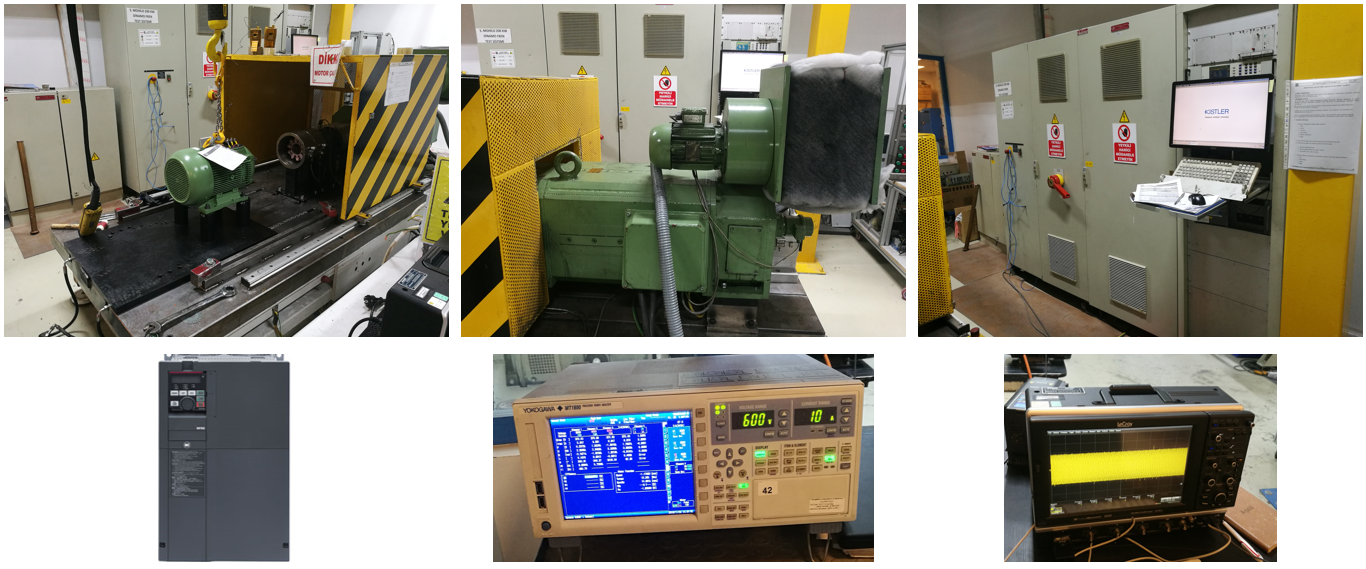
\includegraphics[width=400pt,keepaspectratio=true]{./fig/expsystem.PNG}
	% sekil3.eps: 0x0 pixel, 300dpi, 0.00x0.00 cm, bb=14 14 1155 740
	\caption{Experiment setup, courtesy of WAT Motor Co.}	
	\label{experiment}
\end{figure}

\begin{table*}[h]
	{\setlength{\tabcolsep}{12pt}
		\caption{Equipments used in experimental-setup.}
		\begin{center}
			\vspace{-6mm}
			\begin{tabular}{c}
				\hline \\[-2.45ex] \hline \\[-2.1ex]
				Equipment\\
				\hline \\[-1.8ex]
				Kistler 200 kW Dynamometer  \\
				Yokogawa Power Analyzer  \\
				Teledyne LeCroy Oscilloscope  \\
				WAT-11 kW Induction Motors   \\
				WAT-WF-80 General Purpose Variable Frequency Driver   \\
				\hline
			\end{tabular}
			\vspace{-6mm}
		\end{center}
		\label{Table3.1}}
\end{table*}

In the experimental studies, the stability of the system was monitored by monitoring the three-phase current and voltage signals on the power analyzer. One phase of the stator supply current of the motor was recorded with a current probe at a sampling frequency of 5 kHz for 10 seconds. In addition, the load torque acting on the motor and the rotor rotation speed of the motor were measured via the dynamometer system.

\begin{figure}[h]
	\centering
	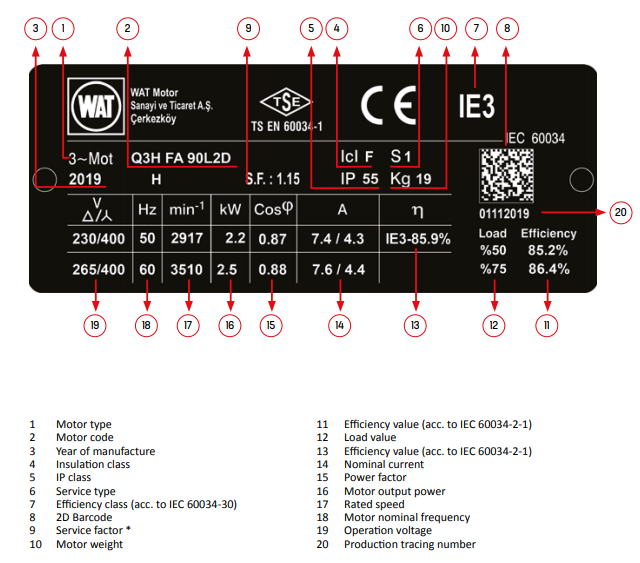
\includegraphics[width=250pt,keepaspectratio=true]{./fig/plate.PNG}
	% sekil3.eps: 0x0 pixel, 300dpi, 0.00x0.00 cm, bb=14 14 1155 740
	\caption{Typical induction motor label, courtesy of WAT Motor Co.}	
	\label{plate}
\end{figure}

\begin{table*}[h]
	{\setlength{\tabcolsep}{12pt}
		\caption{Nominal Values of WAT Motor 3-phase Induction Motor.}
		\begin{center}
			\vspace{-6mm}
			\begin{tabular}{cclccc}
				\hline \\[-2.45ex] \hline \\[-2.1ex]
				\multirow{2}{*}{Voltage ($V$)} & \multicolumn{2}{c}{Power} & \multirow{2}{*}{Speed ($rpm$)} & \multirow{2}{*}	{Current ($A$)} & \multirow{2}{*}{Torque $(N\cdot m)$} \\
				& $(kW)$ & \multicolumn{1}{c}{$(Hz)$} &  &  &  \\
				\hline \\[-1.8ex]
			   	\multicolumn{1}{l}{400/690} & \multicolumn{1}{l}{11} & 50 & \multicolumn{1}{l}{1475} & \multicolumn{1}{l}{22.0/12.7} & \multicolumn{1}{l}{71.3}\\
				\hline
			\end{tabular}
			\vspace{-6mm}
		\end{center}
		\label{Table3.2}}
\end{table*}

\begin{figure}[h]
	\centering
	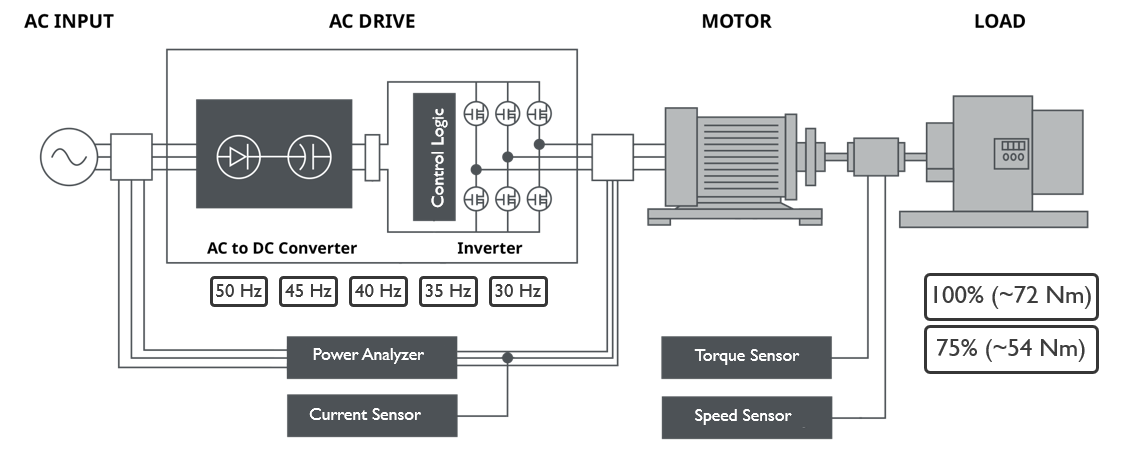
\includegraphics[width=400pt,keepaspectratio=true]{./fig/testsystem.PNG}
	% sekil3.eps: 0x0 pixel, 300dpi, 0.00x0.00 cm, bb=14 14 1155 740
	\caption{Schematic of test system.}	
	\label{schematic}
\end{figure}

Experimental studies were carried out at a rated load of 72 Nm and a frequency of 30, 35, 40, 45 and 50 Hz at 54 Nm, which is 75\% of the rated load, by applying the v/f control method over the VFD. Three motors produced in the same series on the same production line were taken and their data were collected in "healthy" condition under the mentioned conditions. For bearing failure, a fault was artificially created after hammering the drive-end bearing of one of the motors, while for stator failure, the insulation between the two turns in one phase of another motor was eroded. For the last motor, one of the bars in the rotor cage has been drilled for rotor failure. It should also be noted that studies conducted only for two cases in steady-state conditions for the motor as healthy and faulty.

\begin{table*}[h]
	{\setlength{\tabcolsep}{12pt}
		\caption{Table with single row and centered columns.}
		\begin{center}
			\vspace{-6mm}
			\begin{tabular}{ccc}
				\hline \\[-2.45ex] \hline \\[-2.1ex]
				Fault Type & Frequency ($Hz$) & Load $(N\cdot m)$ \\
				\hline \\[-1.8ex]
				Bearing & 30 & $\approx$ 72  \\
				Stator turn-turn & 35 & $\approx$ 54  \\
				Broken Rotor Bar & 40 &  \\
				& 45 &   \\
				& 50 &   \\
				\hline
			\end{tabular}
			\vspace{-6mm}
		\end{center}
		\label{Table3.3}}
\end{table*}

Another issue to be considered while collecting data is the amount of data required to see the effects of failure. In the experiments, the mechanical speed of the rotor varies between 857 and 1472 rpm in proportion to the reference control command applied. According to equation the given in \ref{data} \cite{shenfield2020novel}, approximately 200 data points are taken per revolution of the rotor shaft with 5 kHz sampling frequency and sampling time of 10 seconds, a window width of 50,000 data points, fault impacts expected to be easily captured.

\begin{equation}
	\text{Number of Data Points} = \displaystyle \frac{60 \cdot \text{Sampling Frequency (Hz)}}{\text{Rotor's Mechanical Speed}}
	\label{data}
\end{equation}

In data analysis, studies were carried out in time and frequency domains. In the time domain, the stator supply currents are studied in raw (no-prosessing), while in the frequency domain, Welch's power spectral density estimation is applied to the current data. Current signals obtained in 1 second for solid and faulty conditions under different speed and load conditions, as well as 10 times zoomed, are shared in Figure \ref{bearing100} to Figure \ref{rotor75}. In addition, Figures \ref{psdbearing100} to \ref{psdrotor} demonstrate Welch's PSD estimation applied to healthy and faulty conditions of stator currents.

\begin{table*}[h]
	{\setlength{\tabcolsep}{12pt}
		\caption{Input parameters for estimating Welch's PSD.}
		\begin{center}
			\vspace{-6mm}
			\begin{tabular}{cc}
				\hline \\[-2.45ex] \hline \\[-2.1ex]
				Parameter & Value  \\
				\hline \\[-1.8ex]
				Window Type & Hamming    \\
				Overlap (\%) & 50 \\
				Number of DFT Points & 5000  \\
				Sample Rate & 5000    \\
				\hline
			\end{tabular}
			\vspace{-6mm}
		\end{center}
		\label{Table3.4}}
\end{table*}
\pagebreak
\begin{figure}[h]
	\centering
	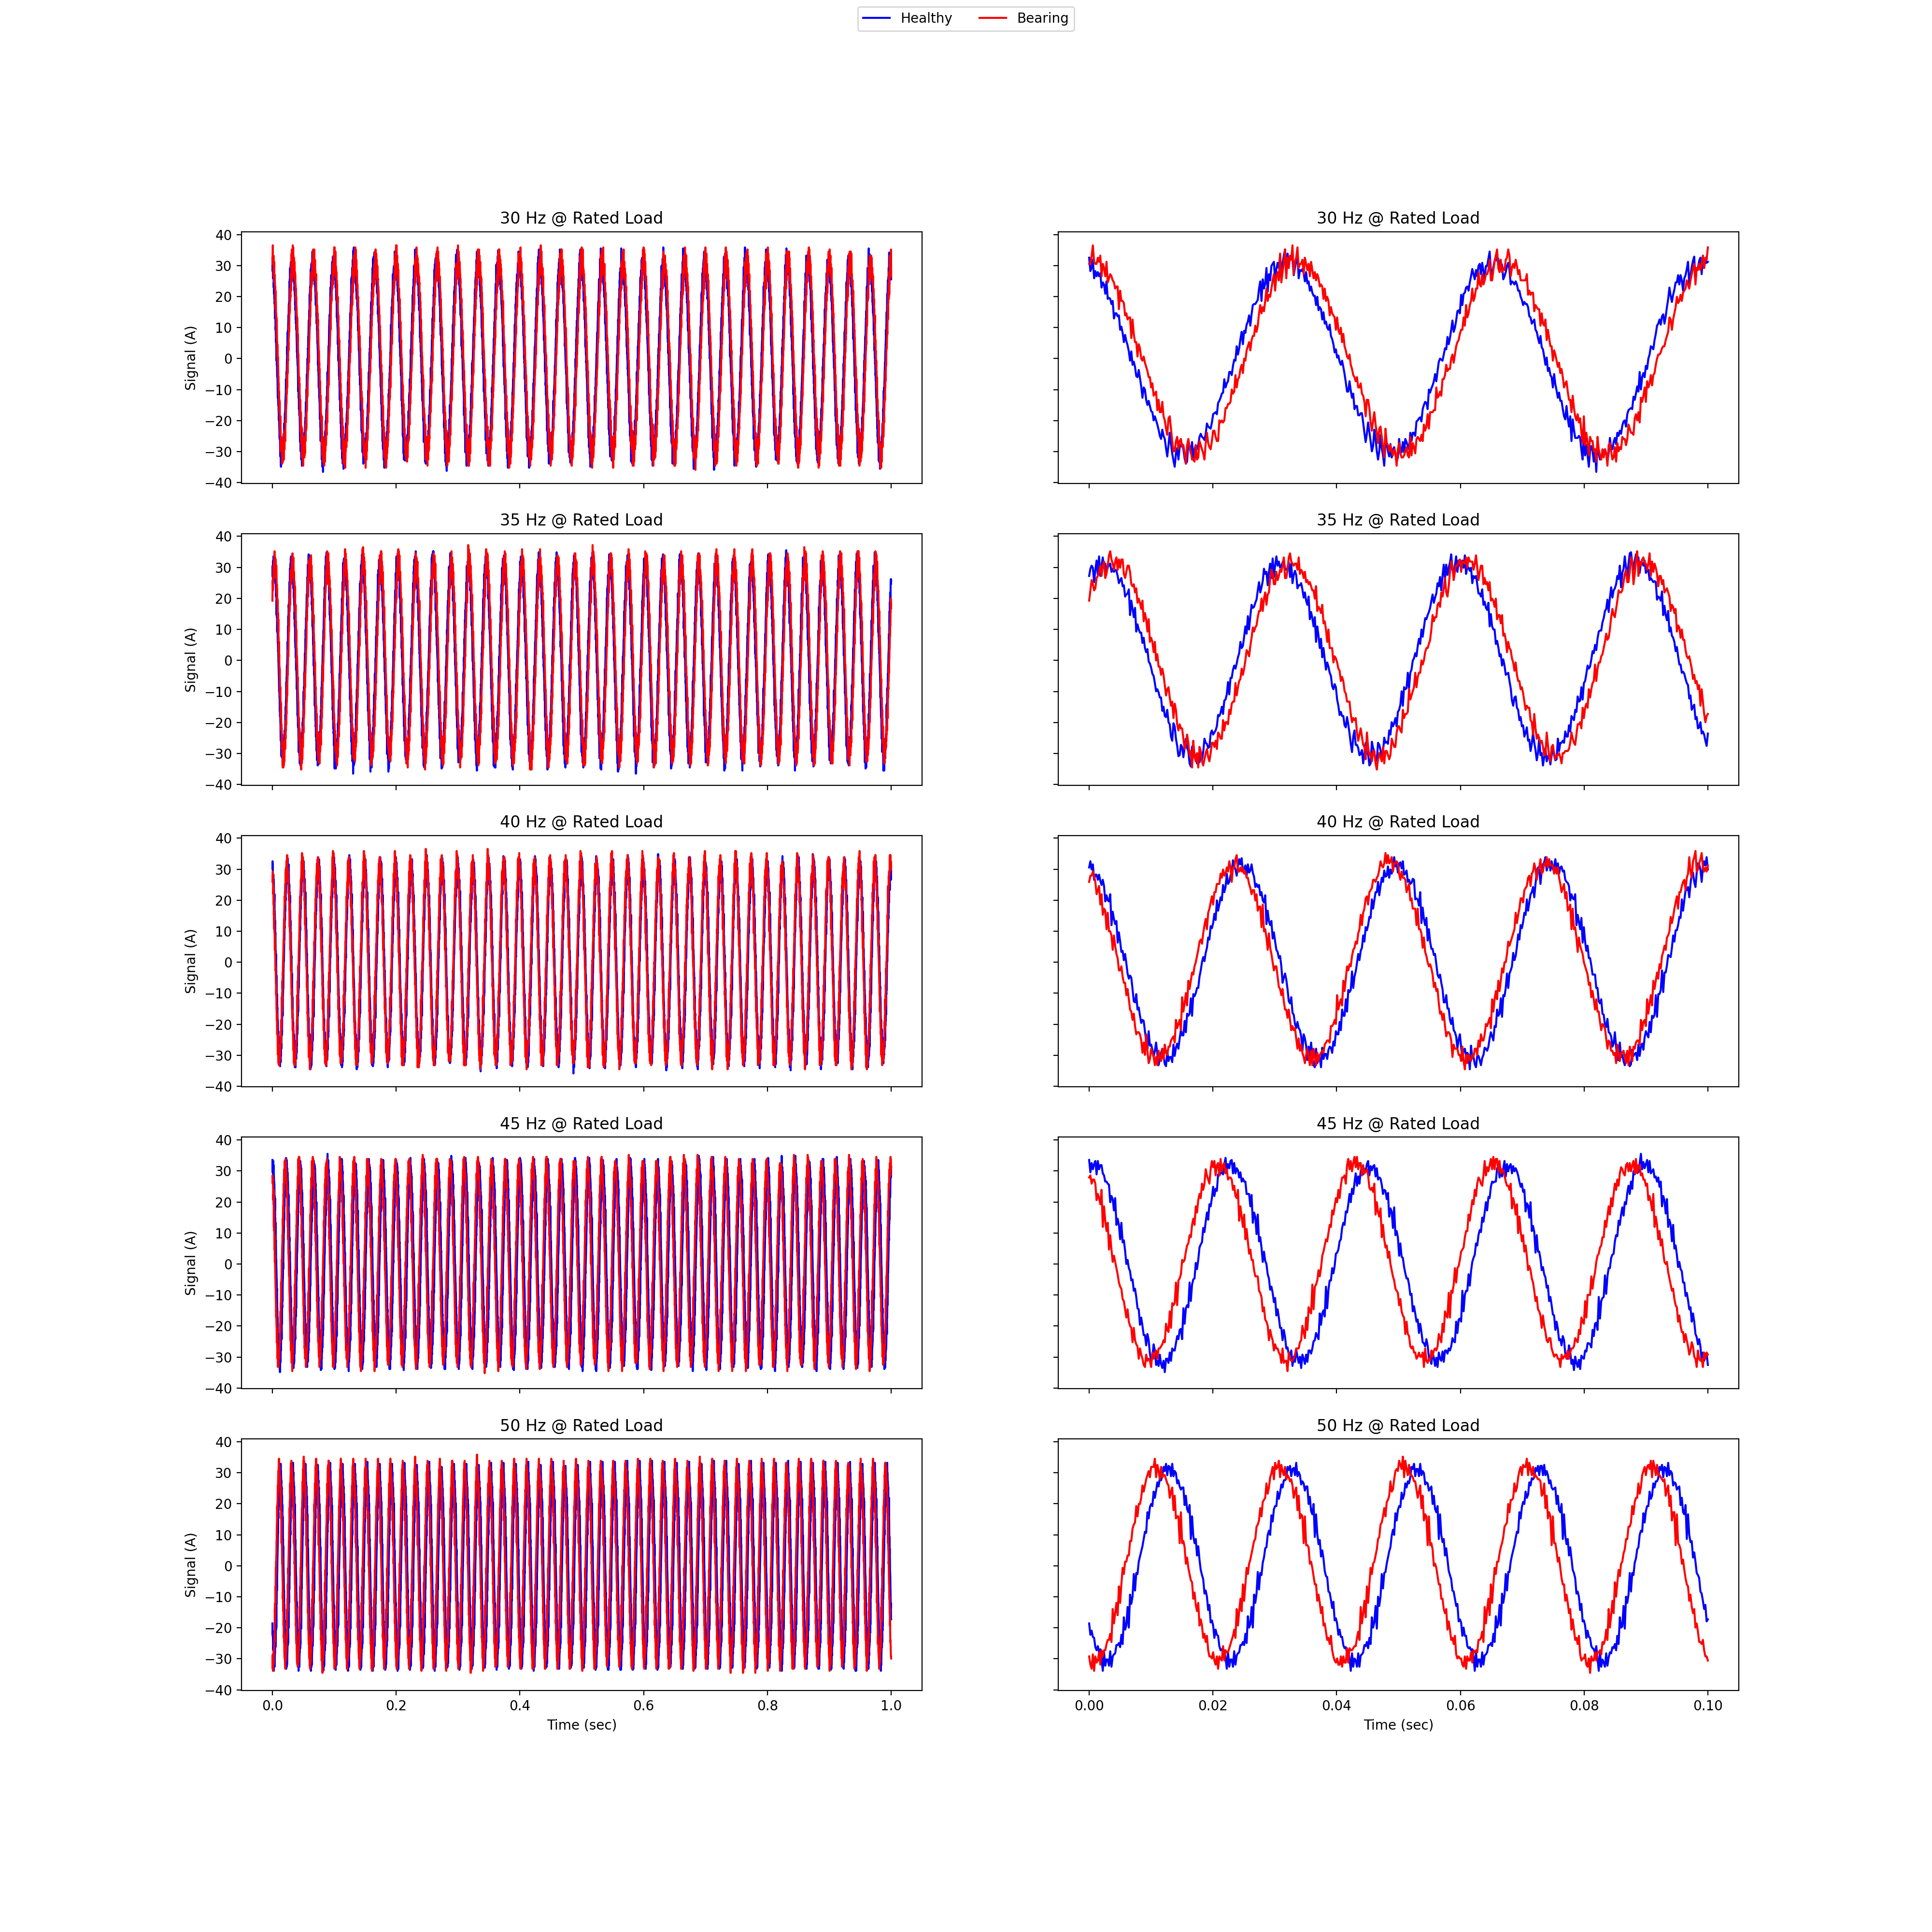
\includegraphics[width=0.8\paperwidth,keepaspectratio=true]{./fig/bearing_100.png}
	% sekil3.eps: 0x0 pixel, 300dpi, 0.00x0.00 cm, bb=14 14 1155 740
	\caption{An example of stator current signals of healthy and bearing-fault motor at rated load.}	
	\label{bearing100}
\end{figure}

\begin{figure}[h]
	\centering
	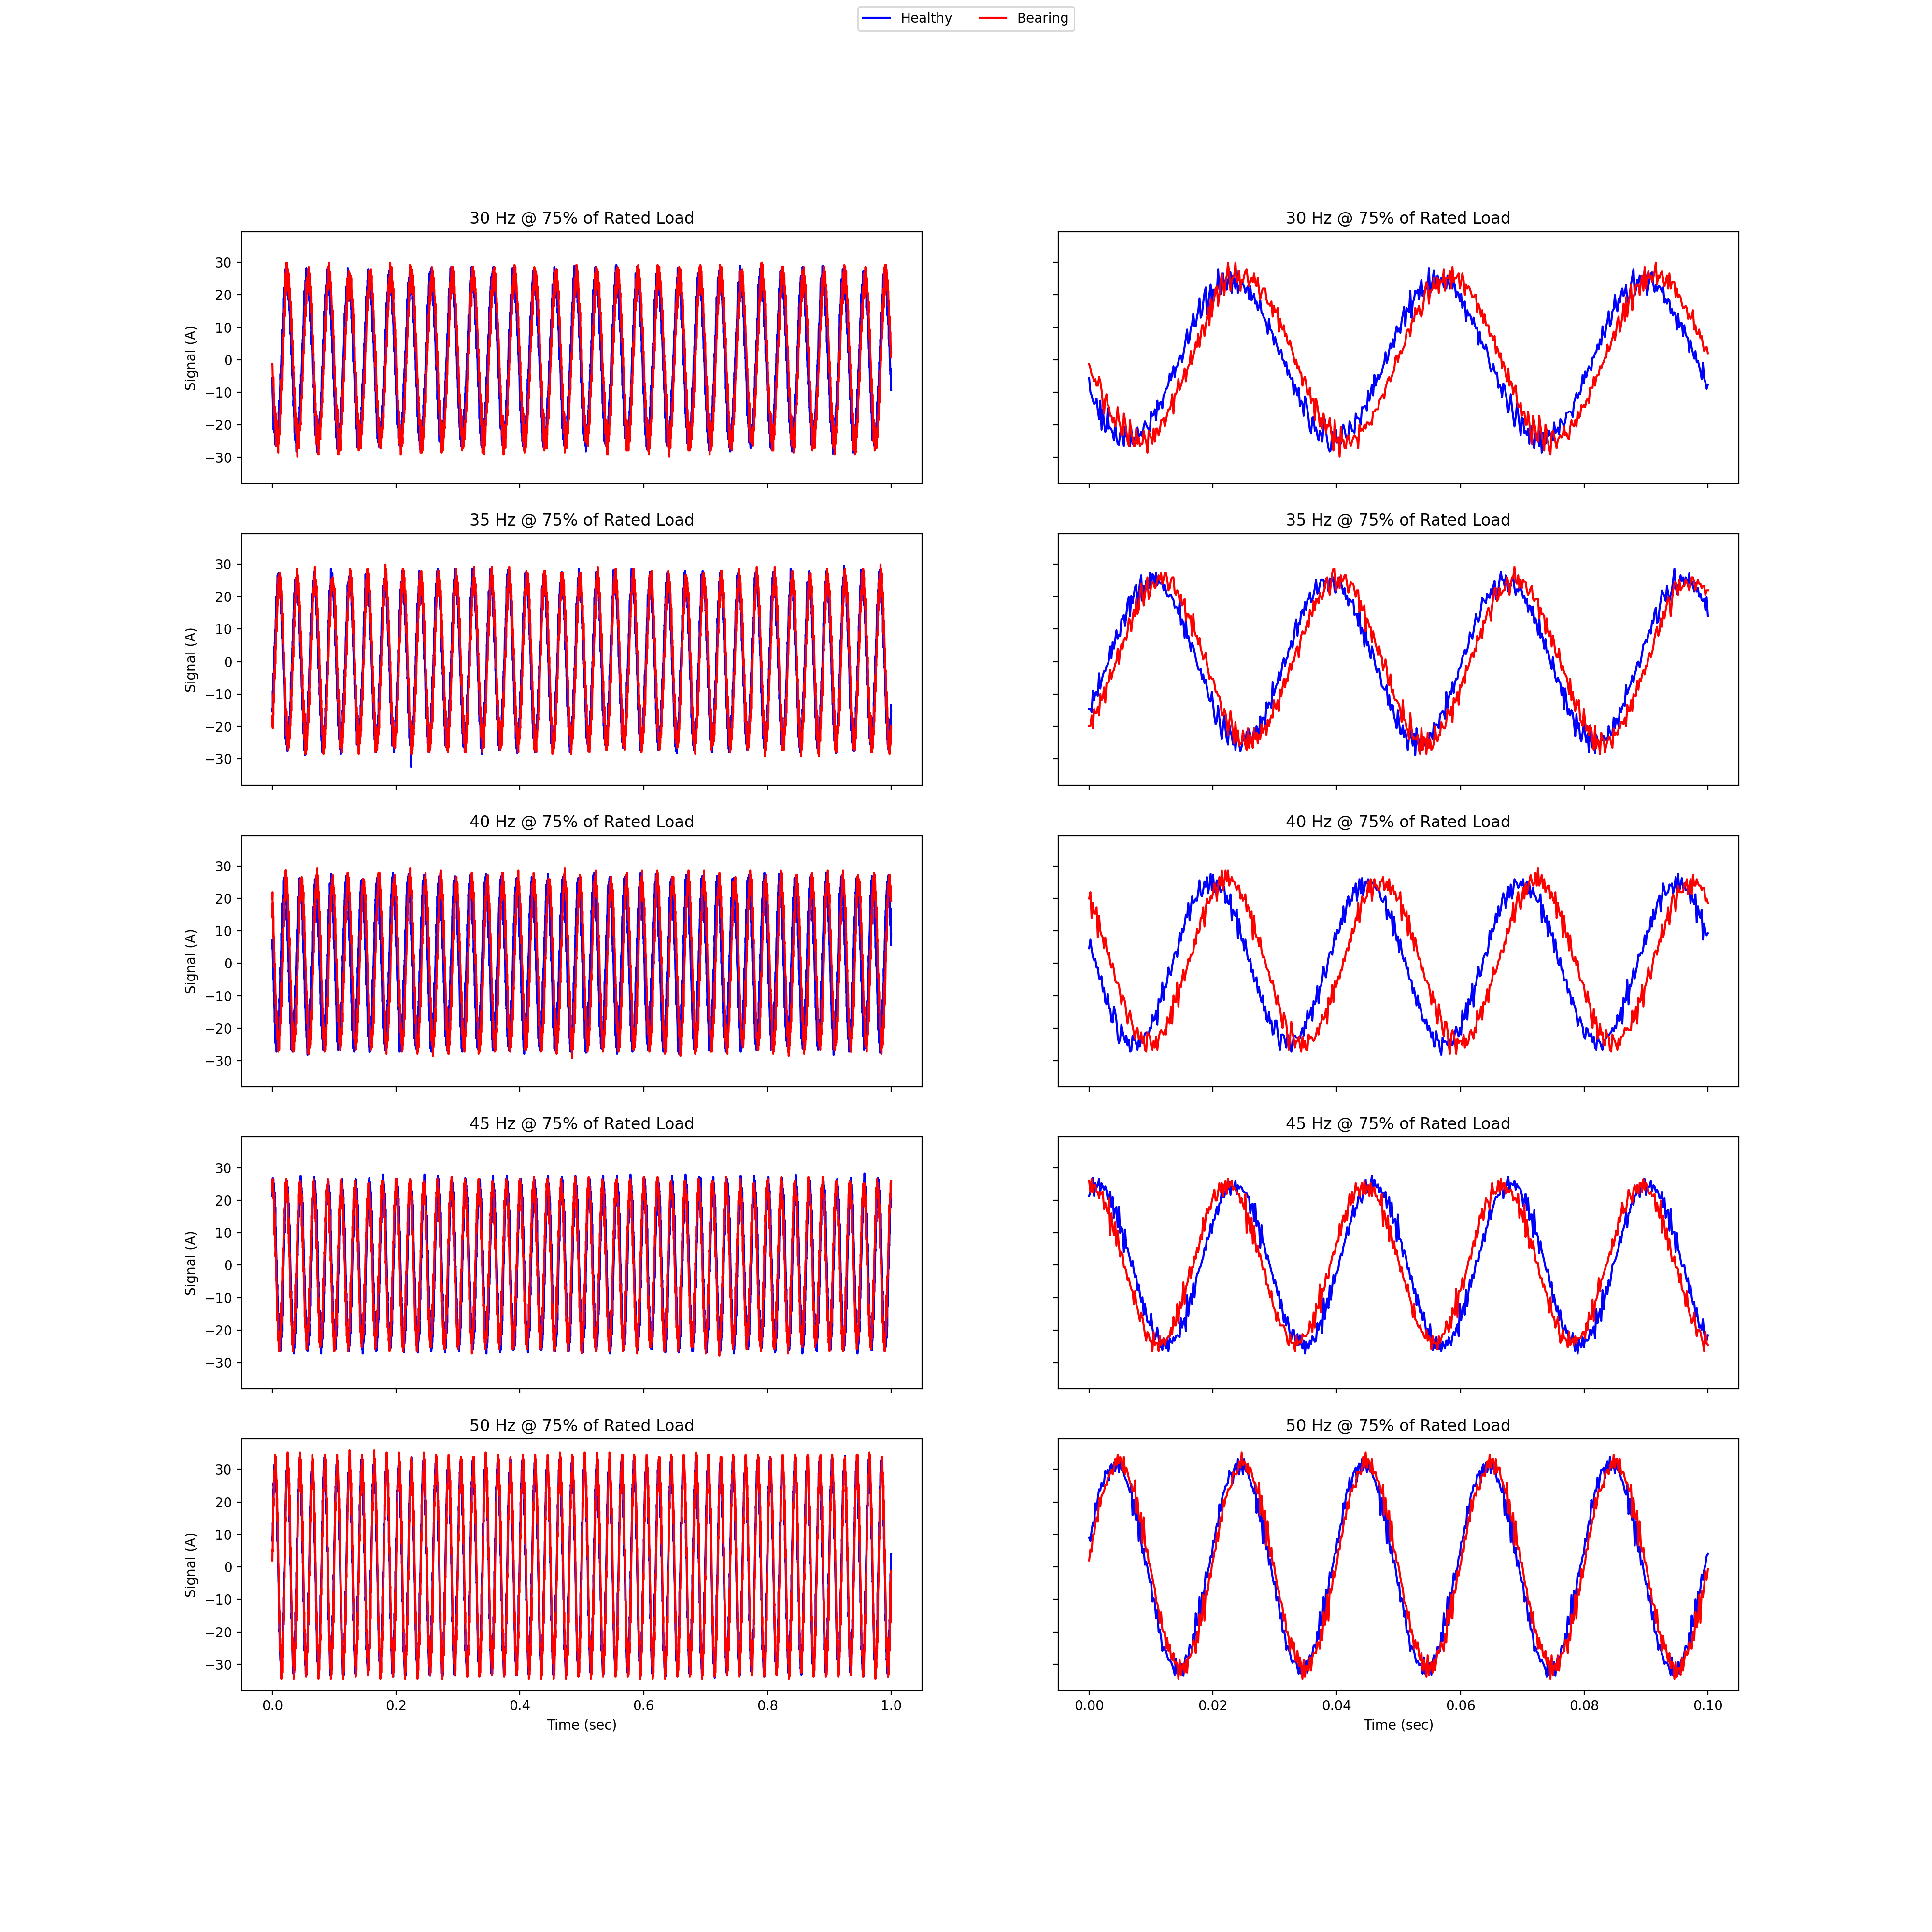
\includegraphics[width=0.8\paperwidth,keepaspectratio=true]{./fig/bearing_75.png}
	% sekil3.eps: 0x0 pixel, 300dpi, 0.00x0.00 cm, bb=14 14 1155 740
	\caption{An example of stator current signals of healthy and bearing-fault motor at $75\%$ of the rated load.}	
	\label{bearing75}
\end{figure}
\pagebreak
\begin{figure}[h]
	\centering
	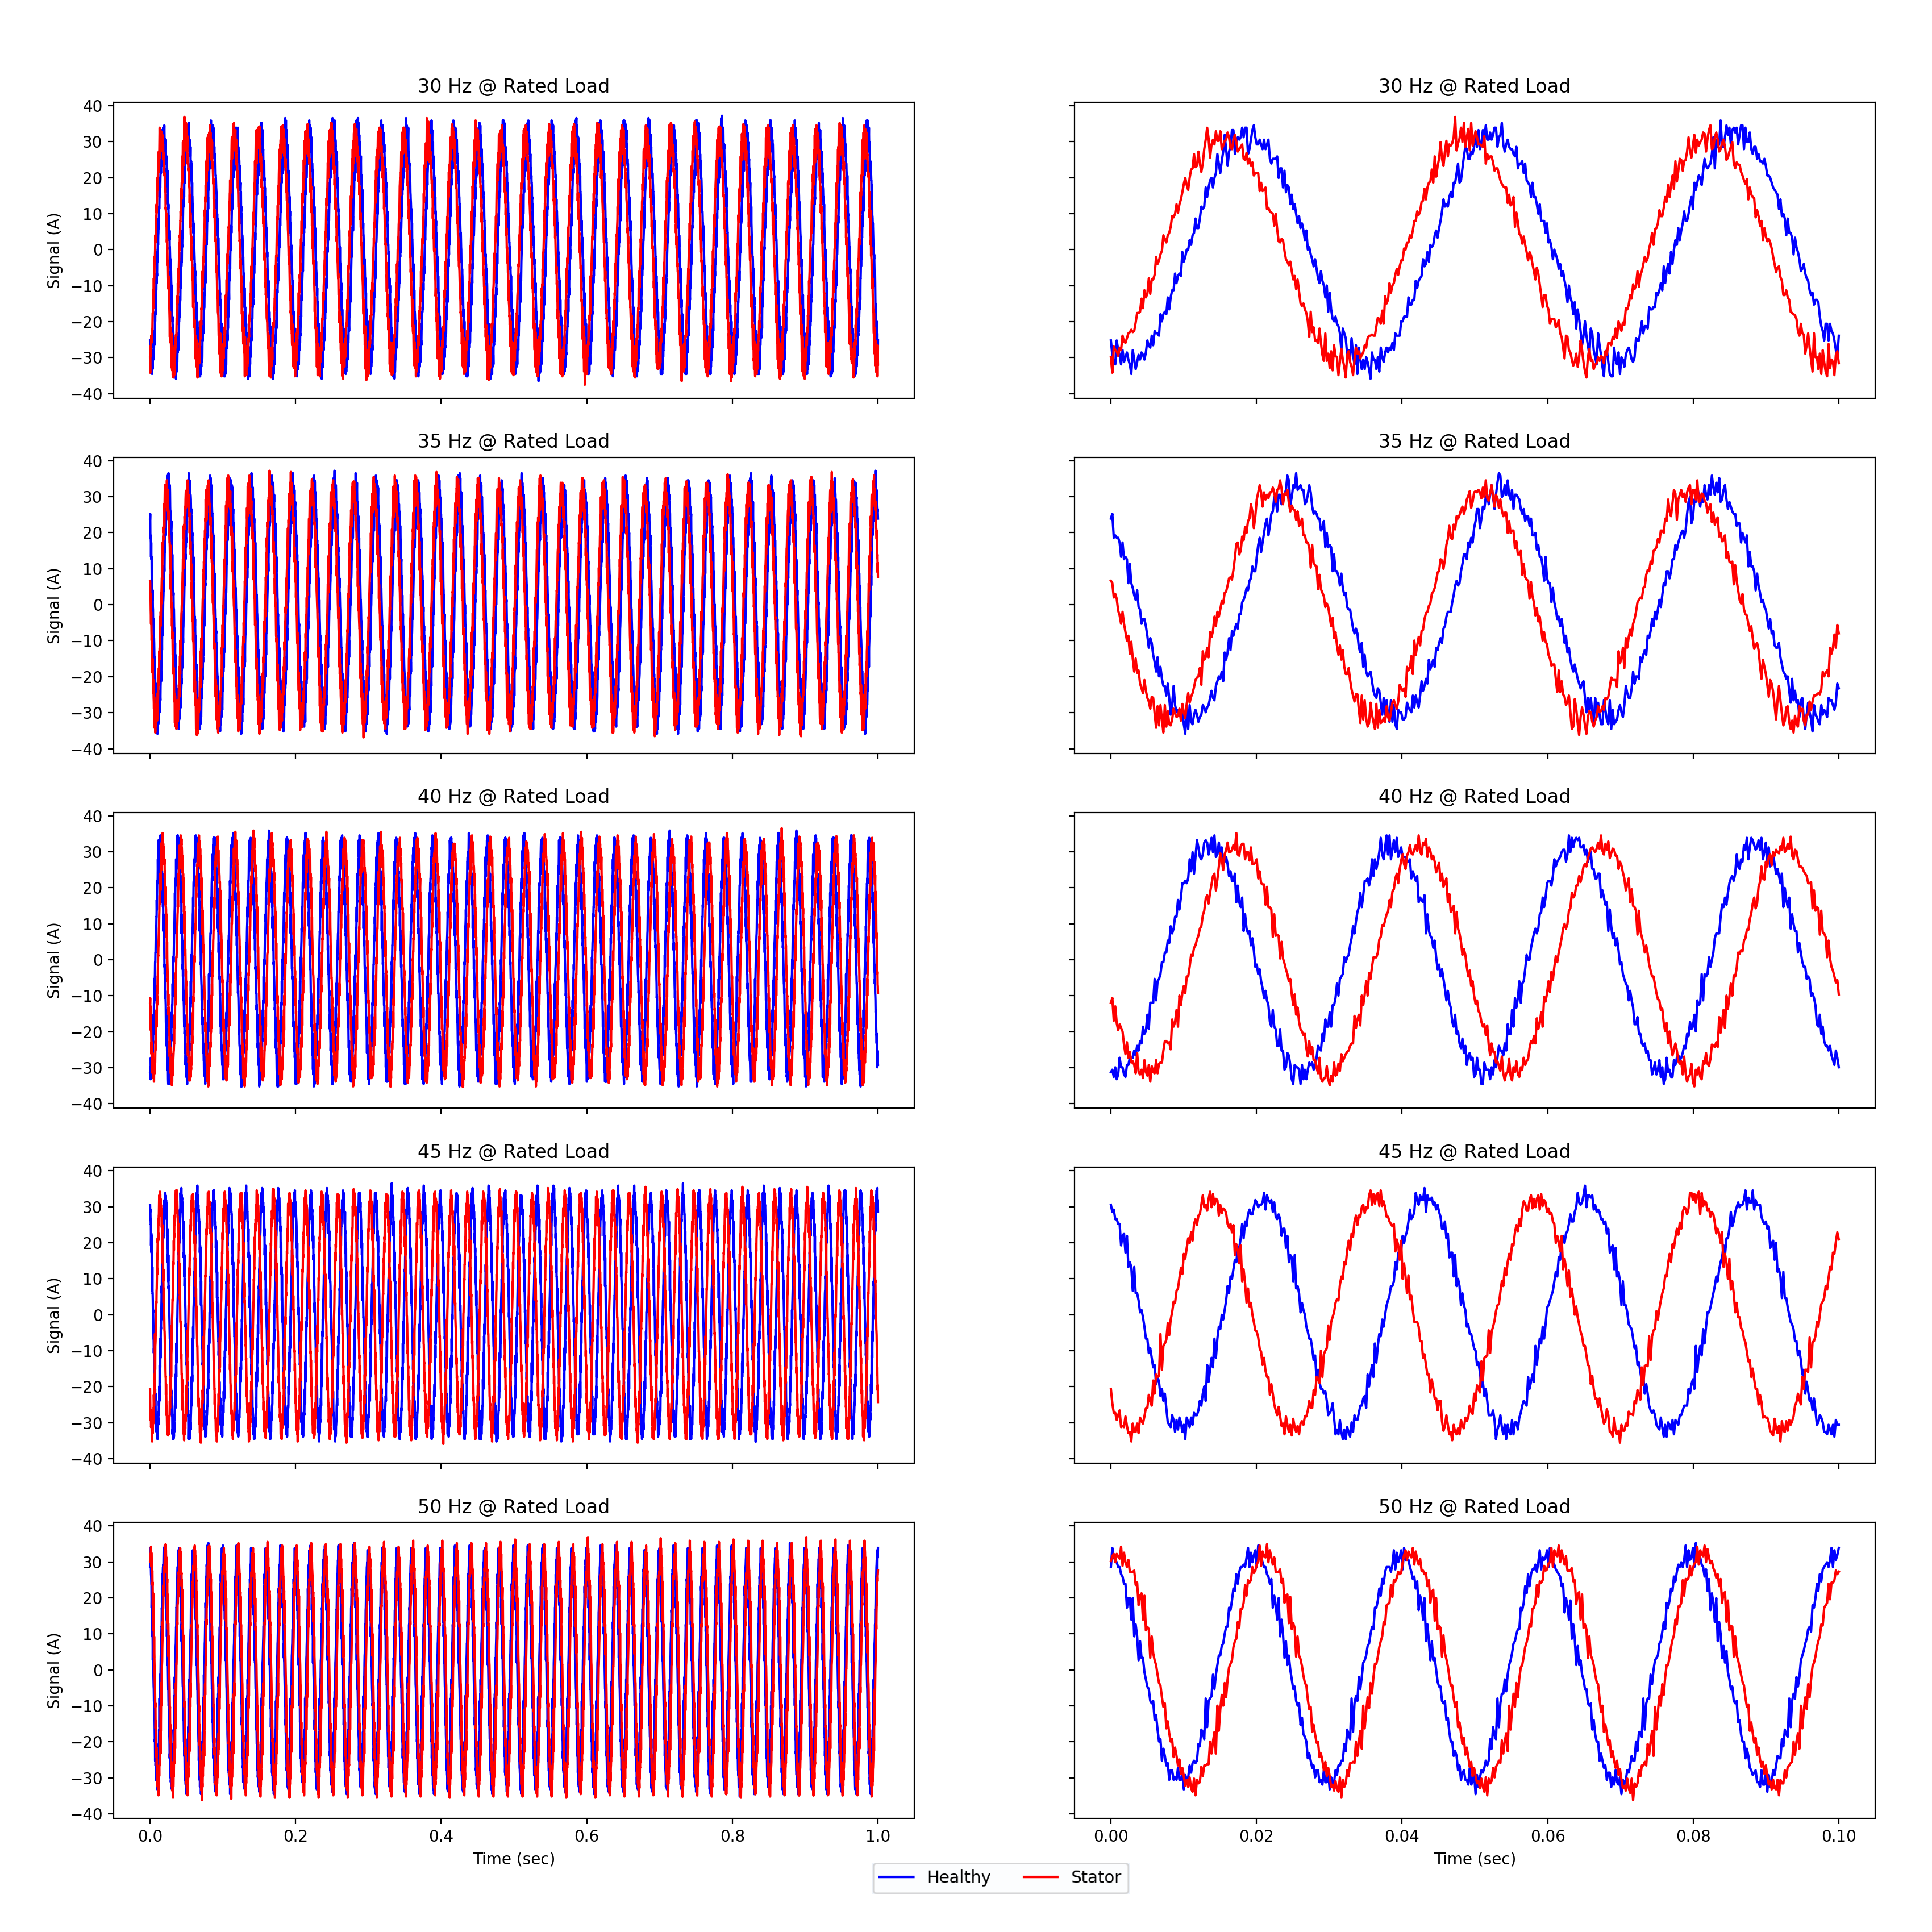
\includegraphics[width=0.8\paperwidth,keepaspectratio=true]{./fig/stator_100.png}
	% sekil3.eps: 0x0 pixel, 300dpi, 0.00x0.00 cm, bb=14 14 1155 740
	\caption{An example of stator current signals of healthy and Stator inter-turn-fault motor at 75$\%$ of the rated load.}	
	\label{stator100}
\end{figure}
\pagebreak
\begin{figure}[h]
	\centering
	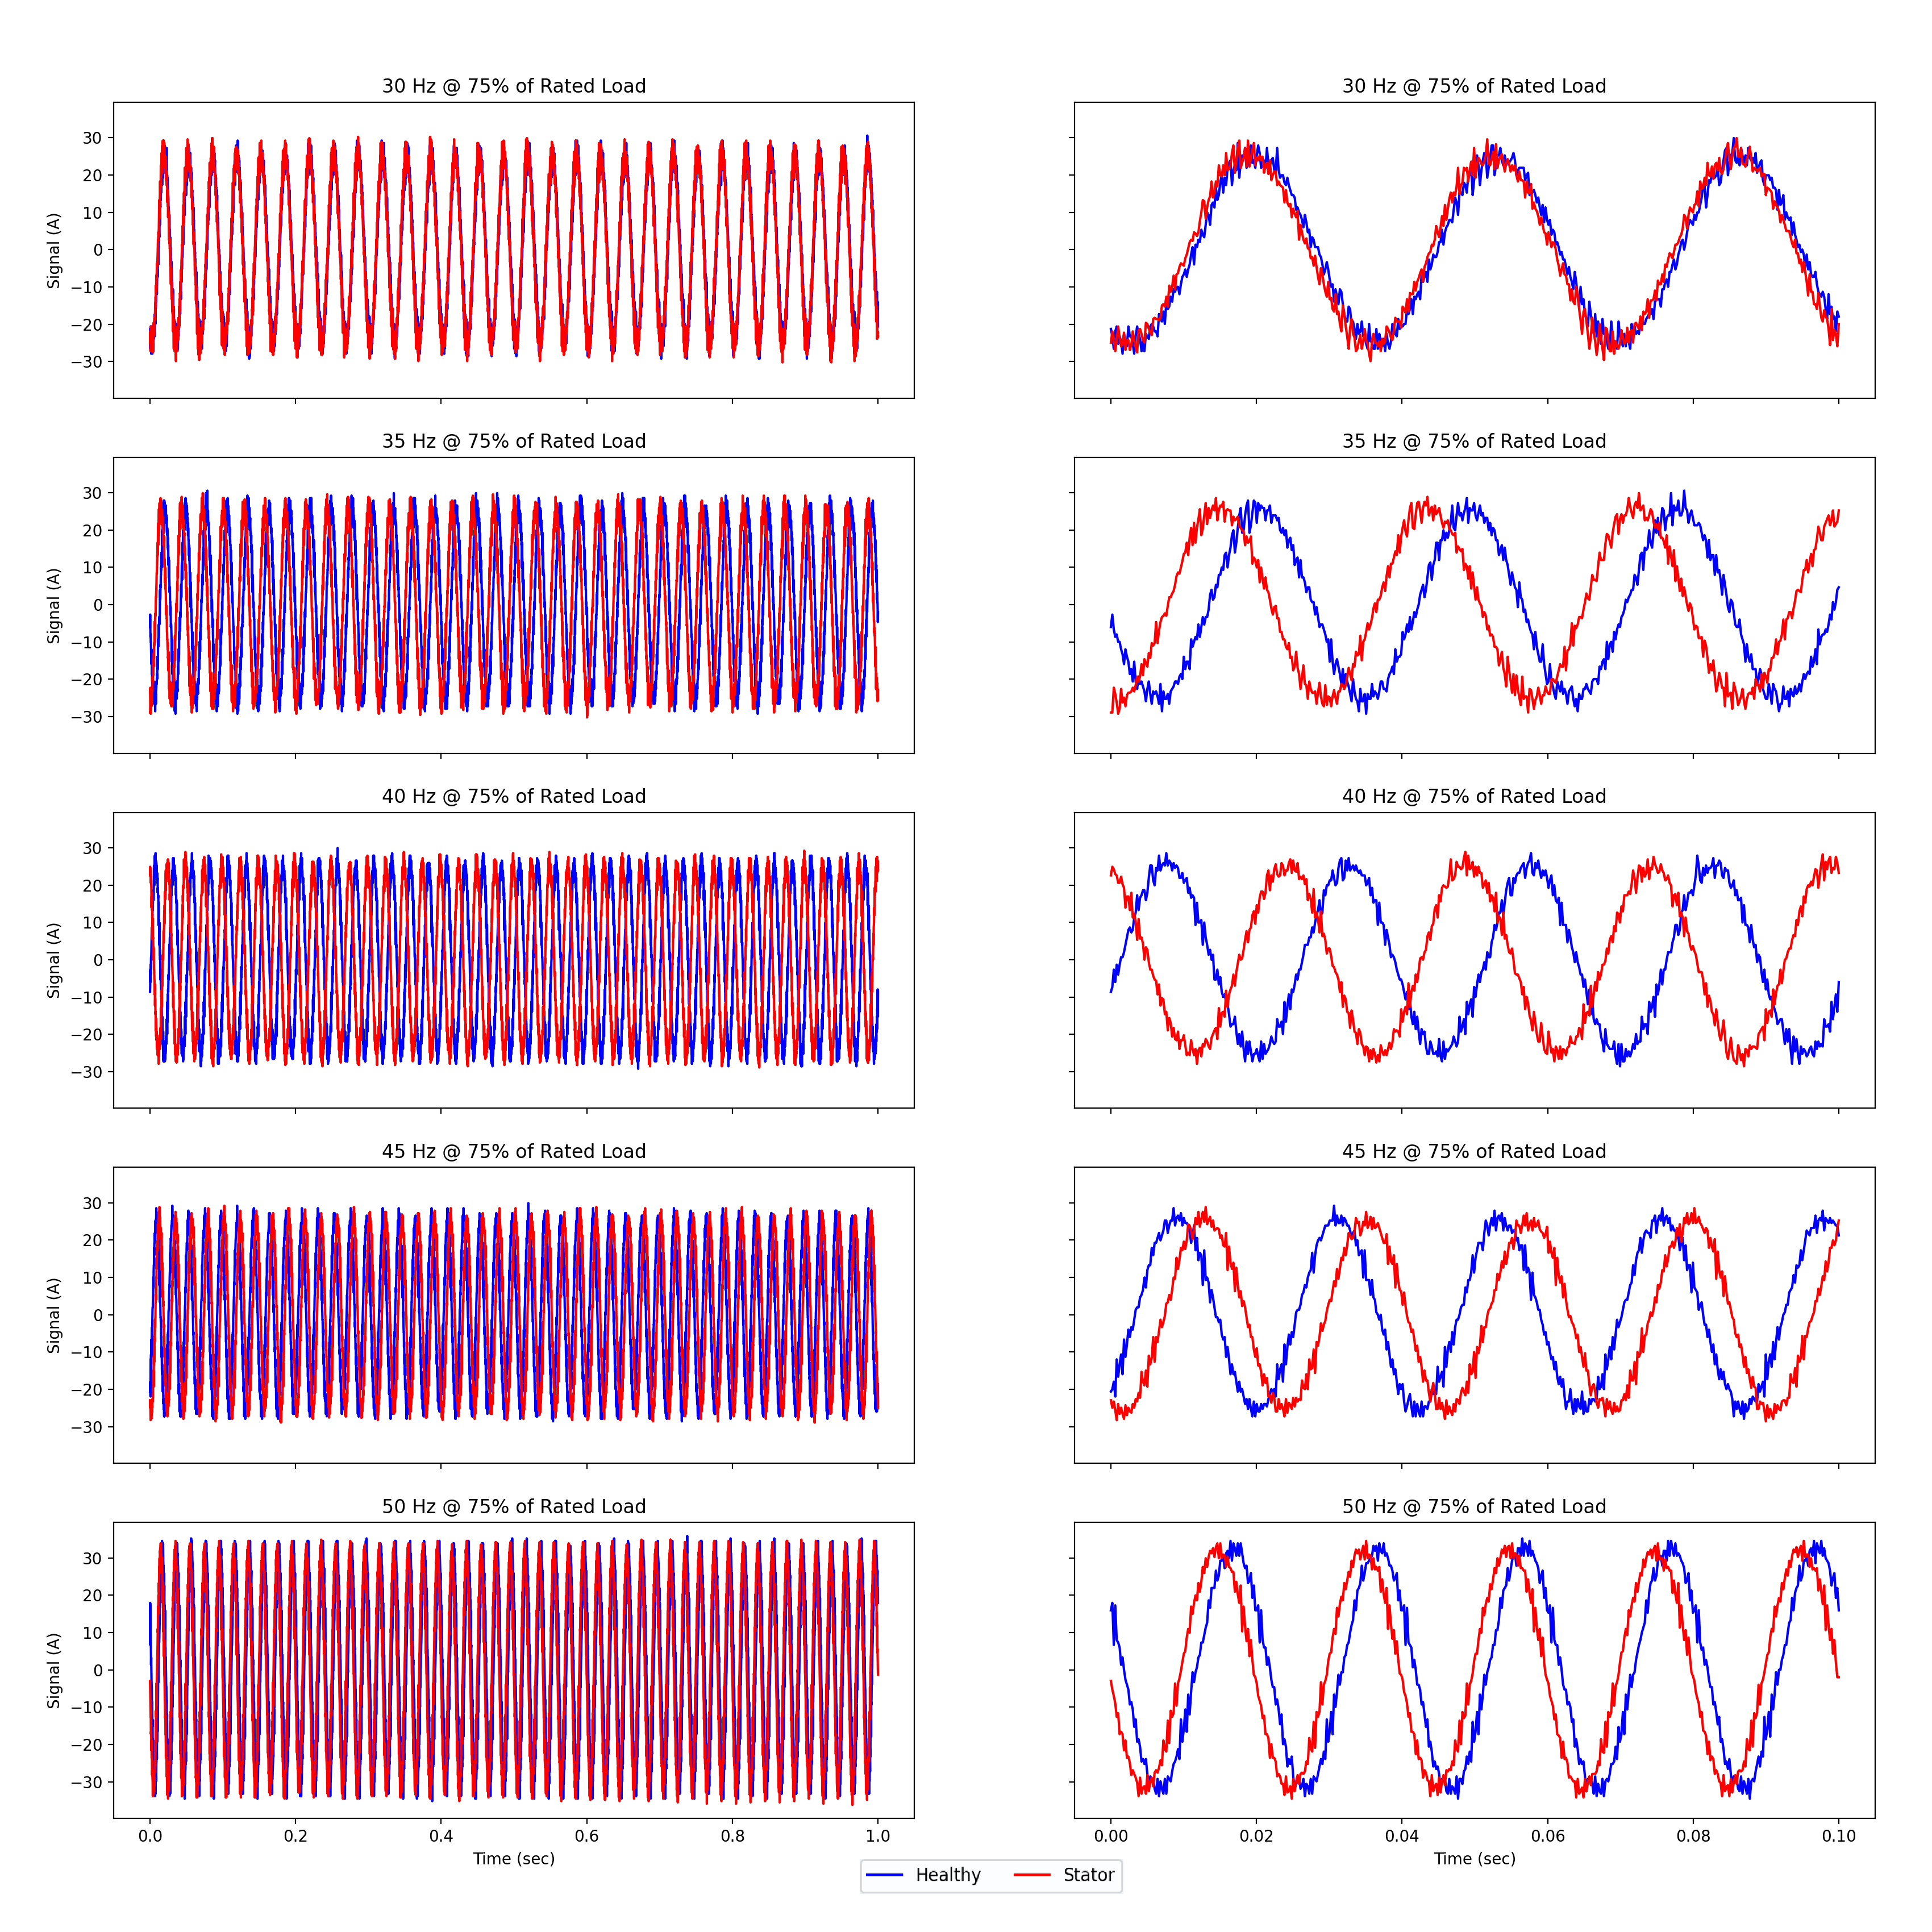
\includegraphics[width=0.8\paperwidth,keepaspectratio=true]{./fig/stator_75.png}
	% sekil3.eps: 0x0 pixel, 300dpi, 0.00x0.00 cm, bb=14 14 1155 740
	\caption{An example of stator current signals of healthy and Stator inter-turn-fault motor at 75$\%$ of the rated load.}	
	\label{stator75}
\end{figure}
\pagebreak
\begin{figure}[h]
	\centering
	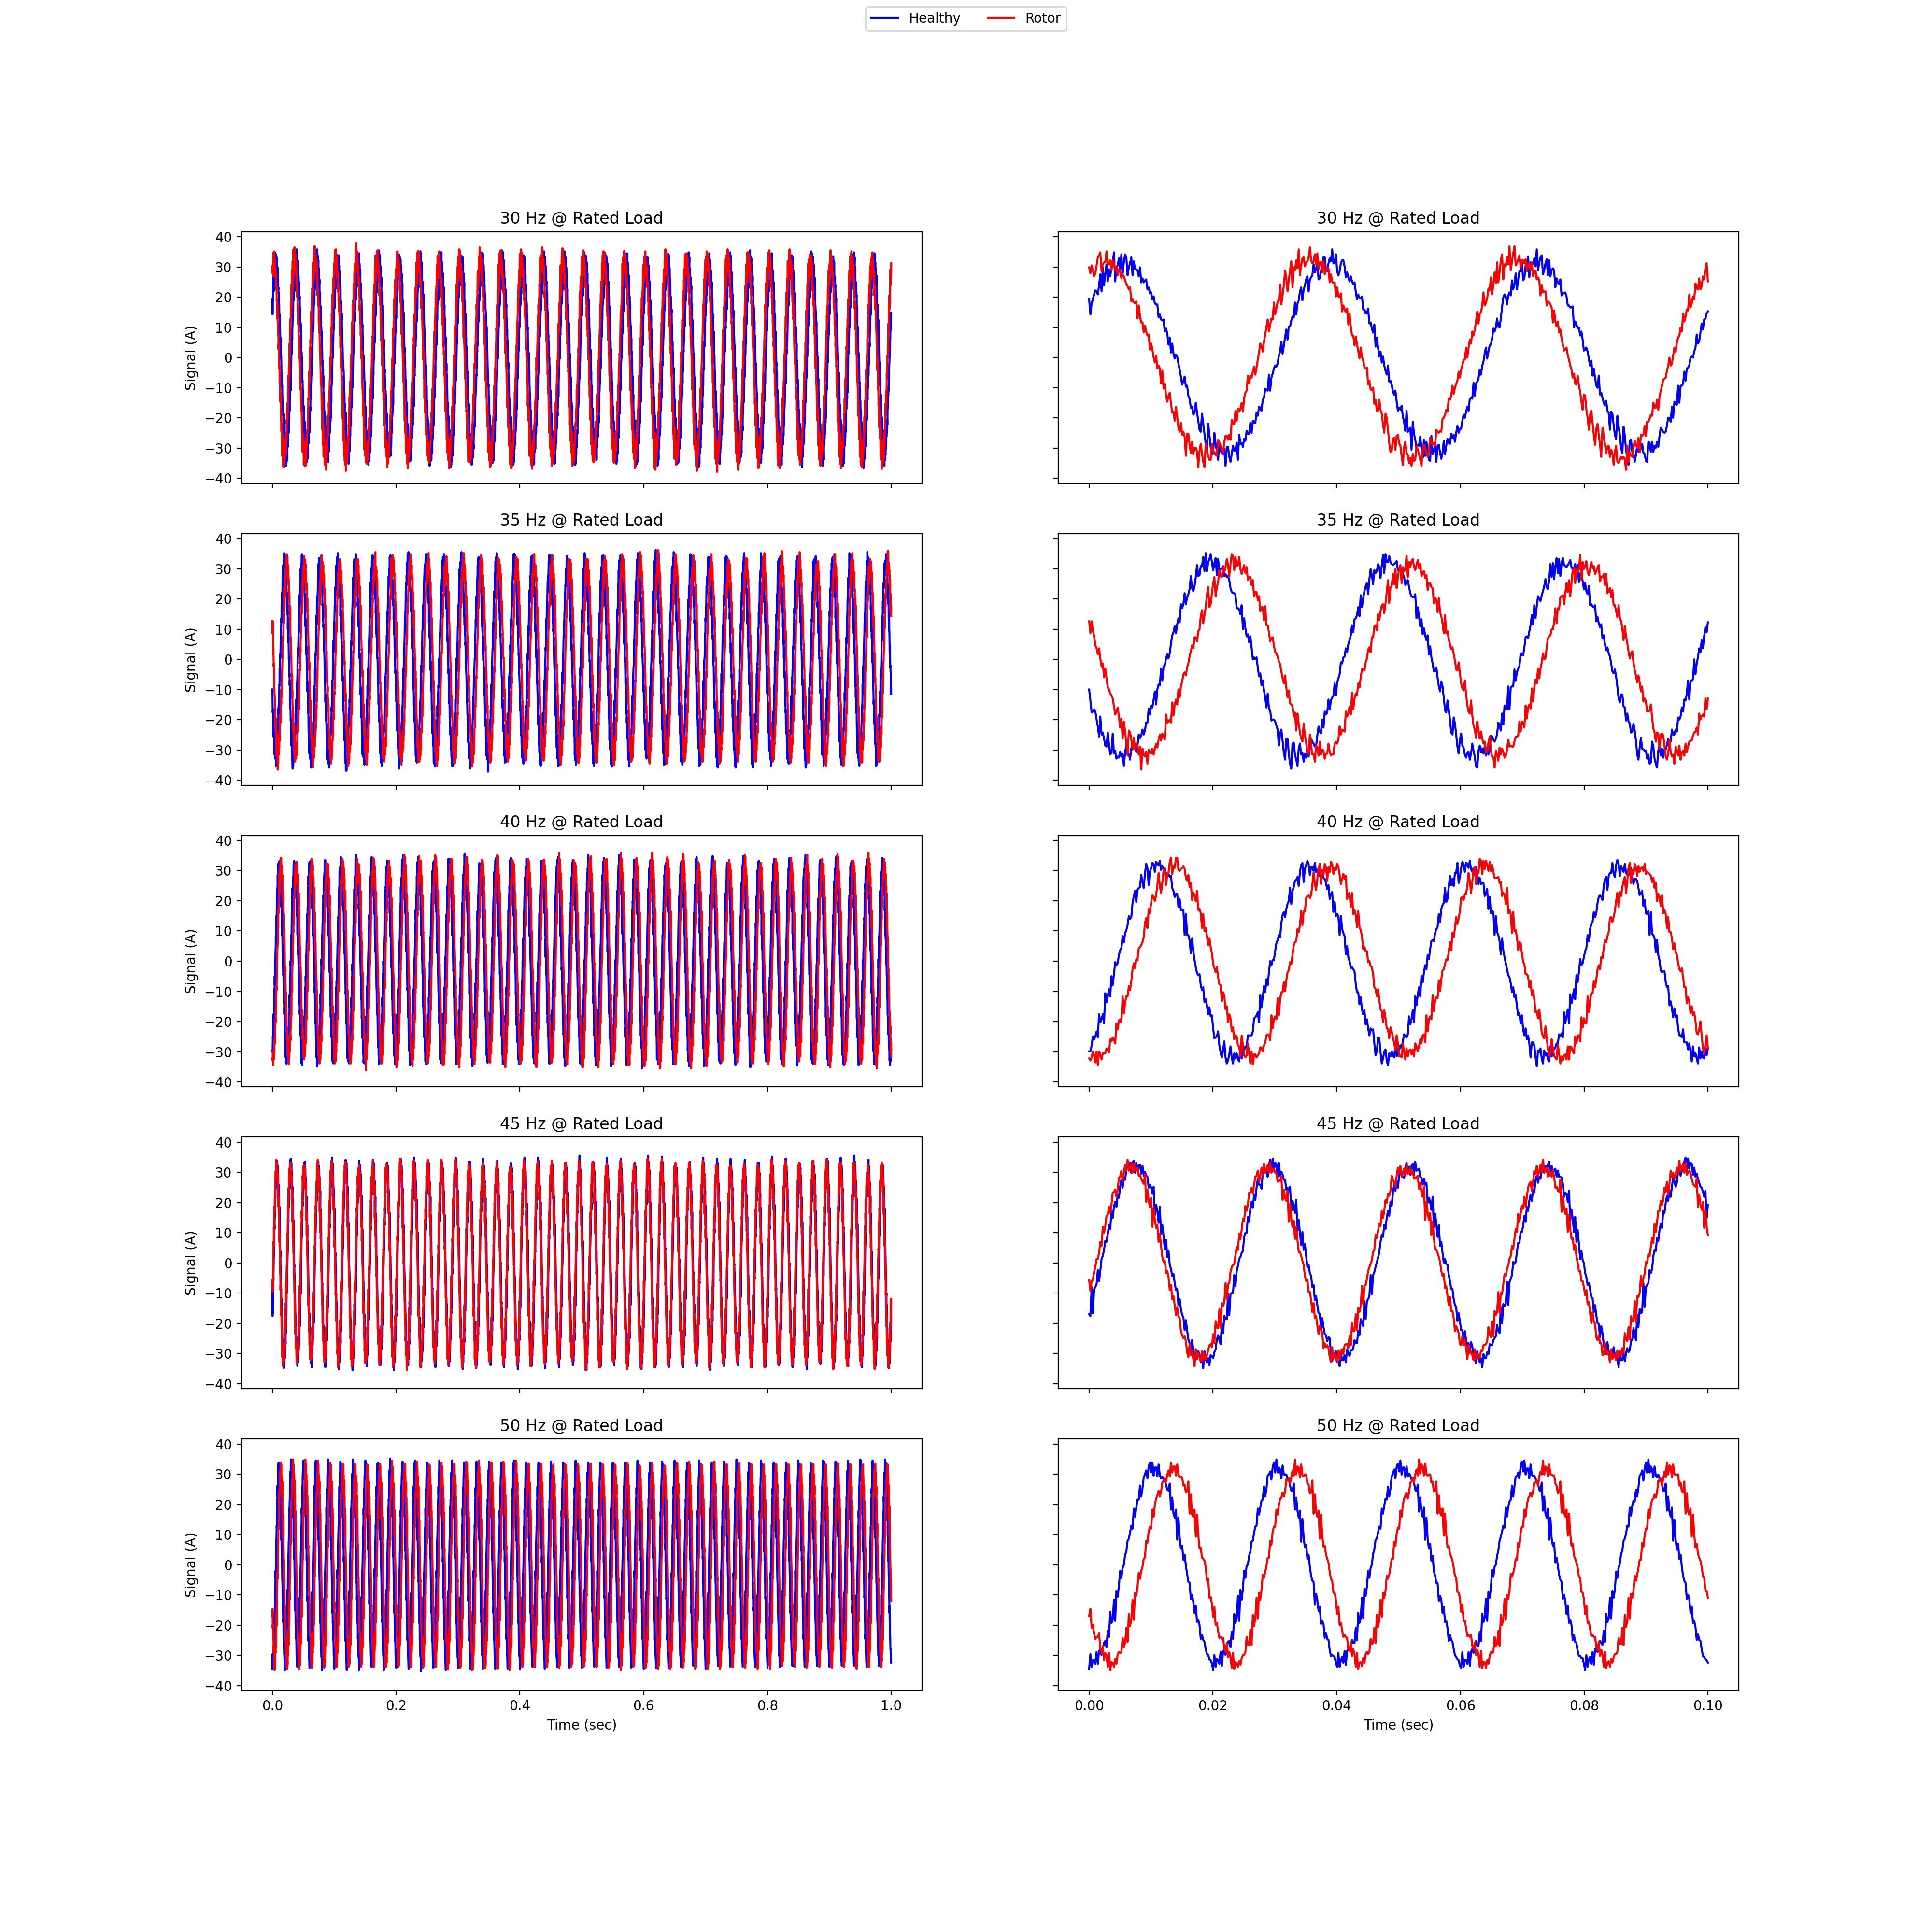
\includegraphics[width=0.8\paperwidth,keepaspectratio=true]{./fig/rotor_100.png}
	% sekil3.eps: 0x0 pixel, 300dpi, 0.00x0.00 cm, bb=14 14 1155 740
	\caption{An example of stator current signals of healthy and 1-Bar Broken Rotor-fault motor at 75$\%$ of the rated load.}	
	\label{rotor100}
\end{figure}
\pagebreak
\begin{figure}[h]
	\centering
	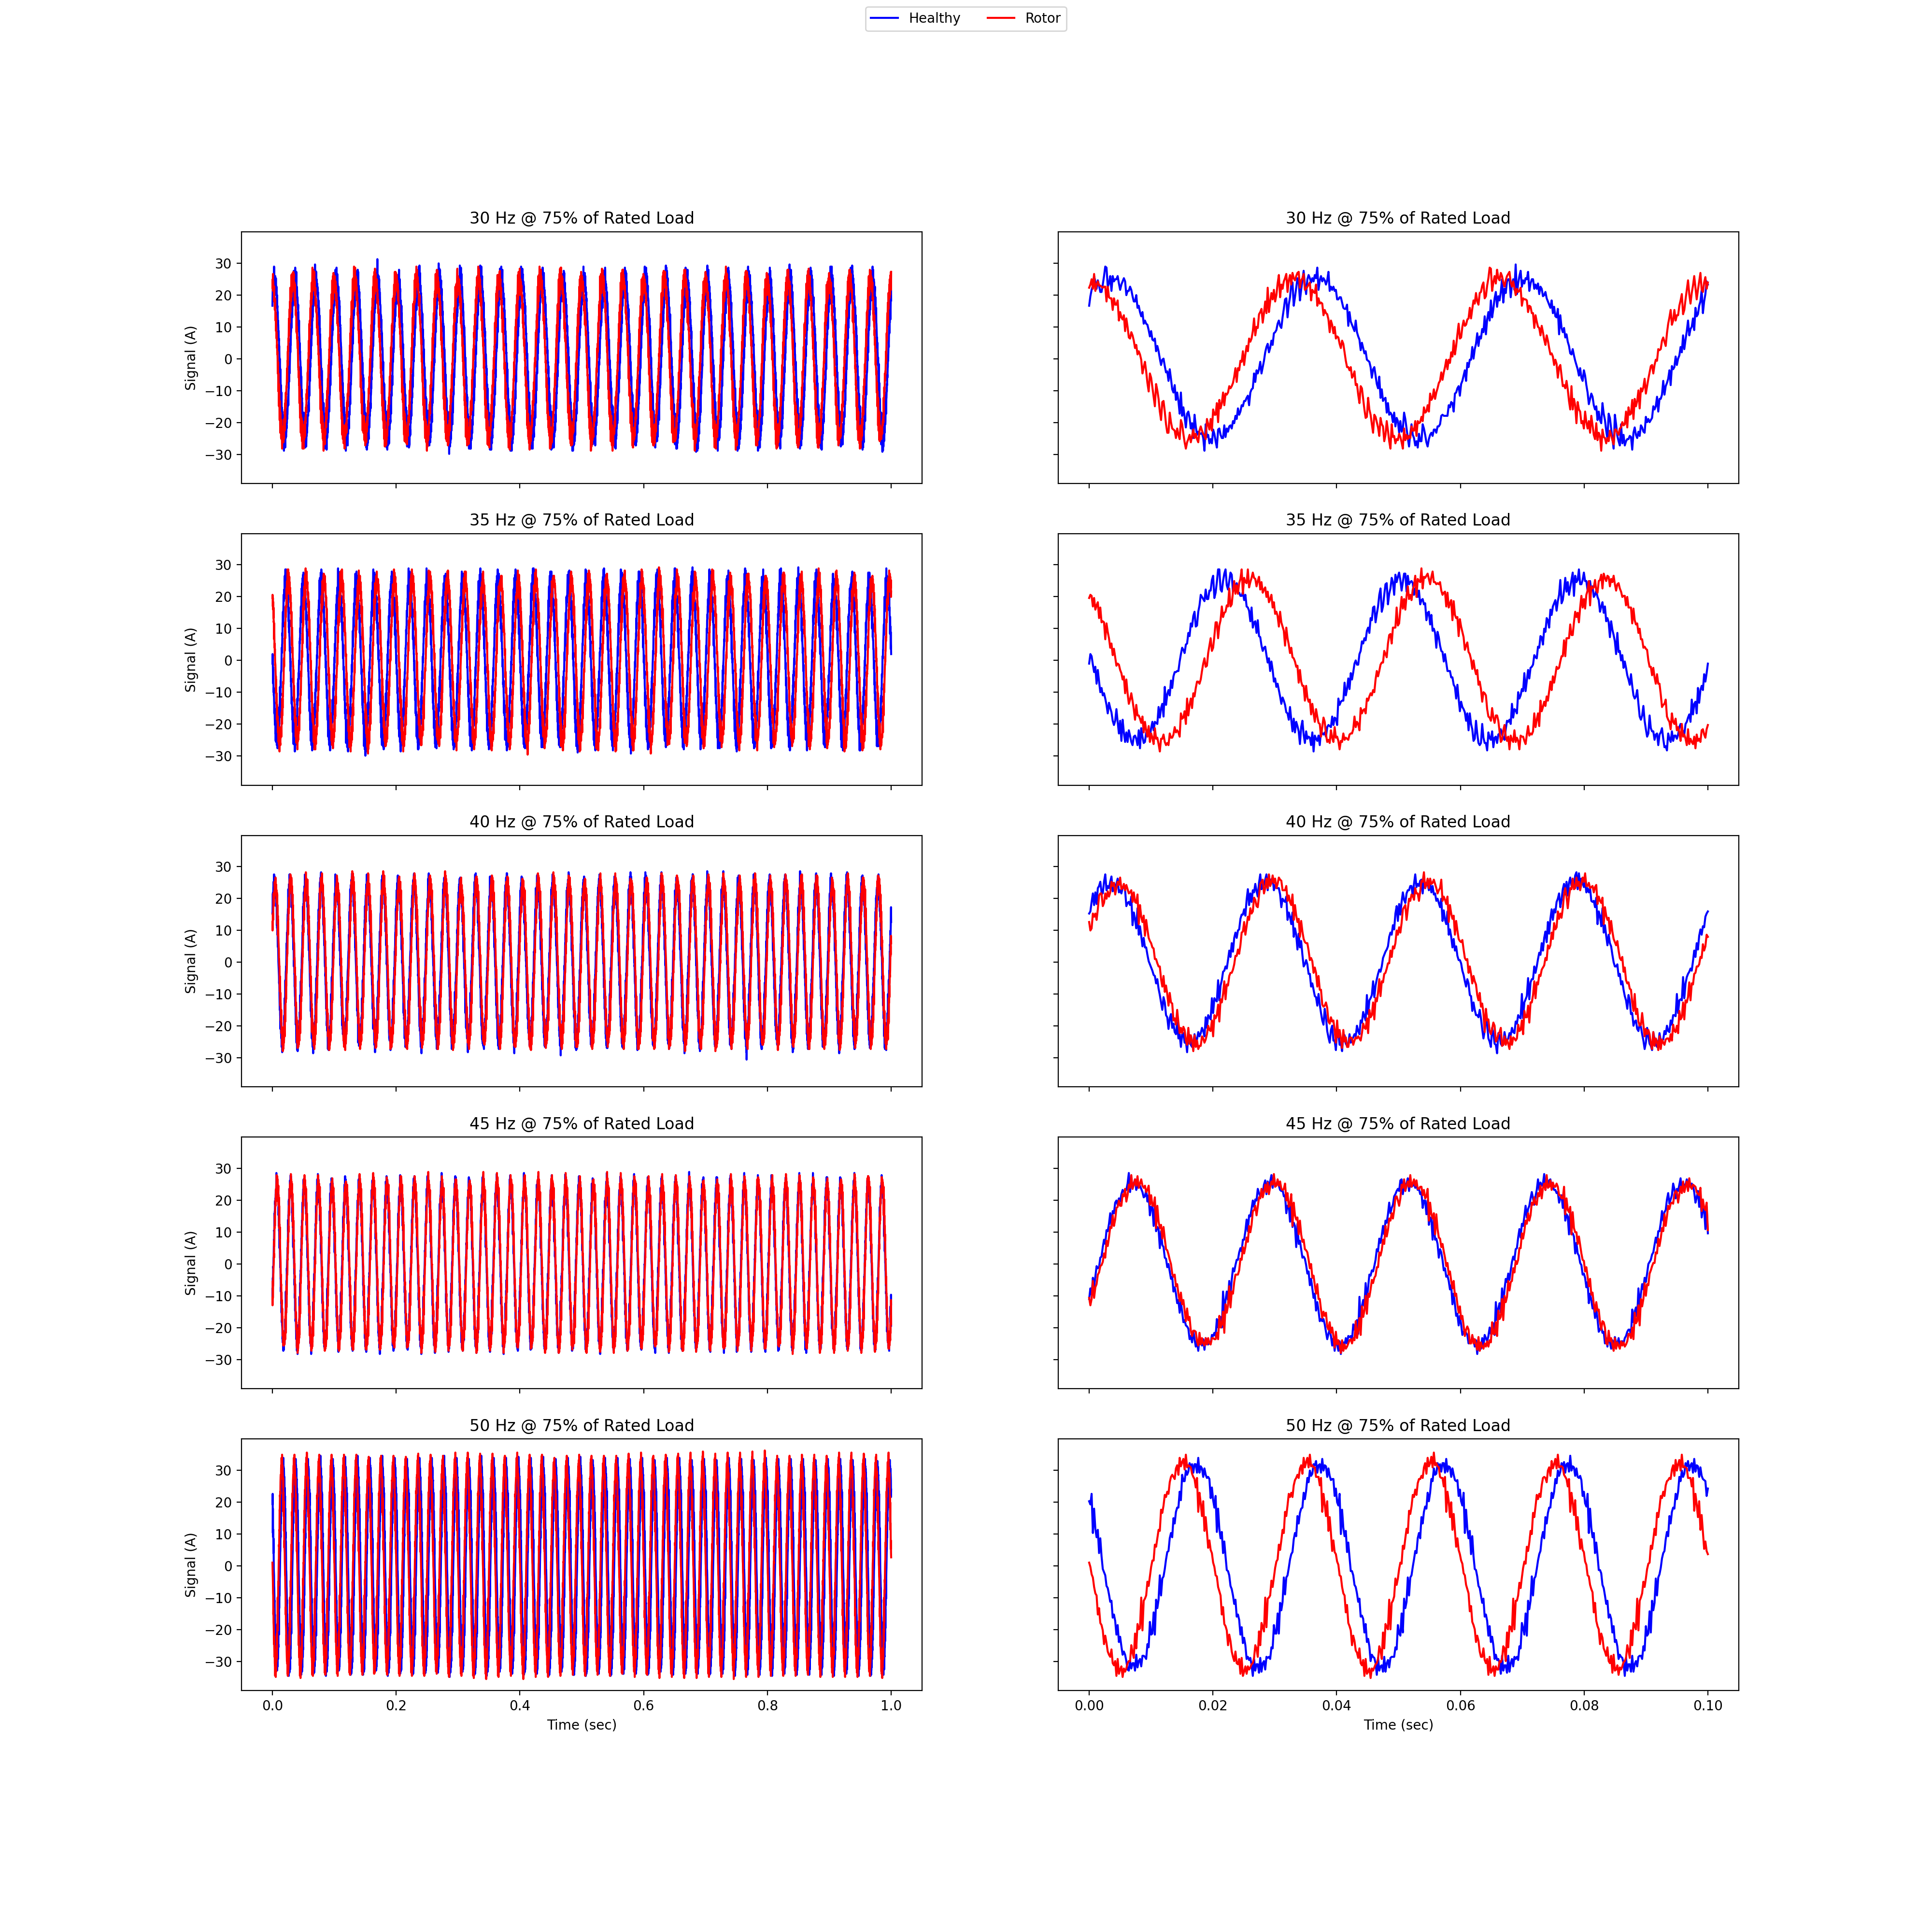
\includegraphics[width=0.8\paperwidth,keepaspectratio=true]{./fig/rotor_75.png}
	% sekil3.eps: 0x0 pixel, 300dpi, 0.00x0.00 cm, bb=14 14 1155 740
	\caption{An example of stator current signals of healthy and 1-Bar Broken Rotor-fault motor at 75$\%$ of the rated load.}	
	\label{rotor75}
\end{figure}
\pagebreak
\begin{figure}[h]
	\centering
	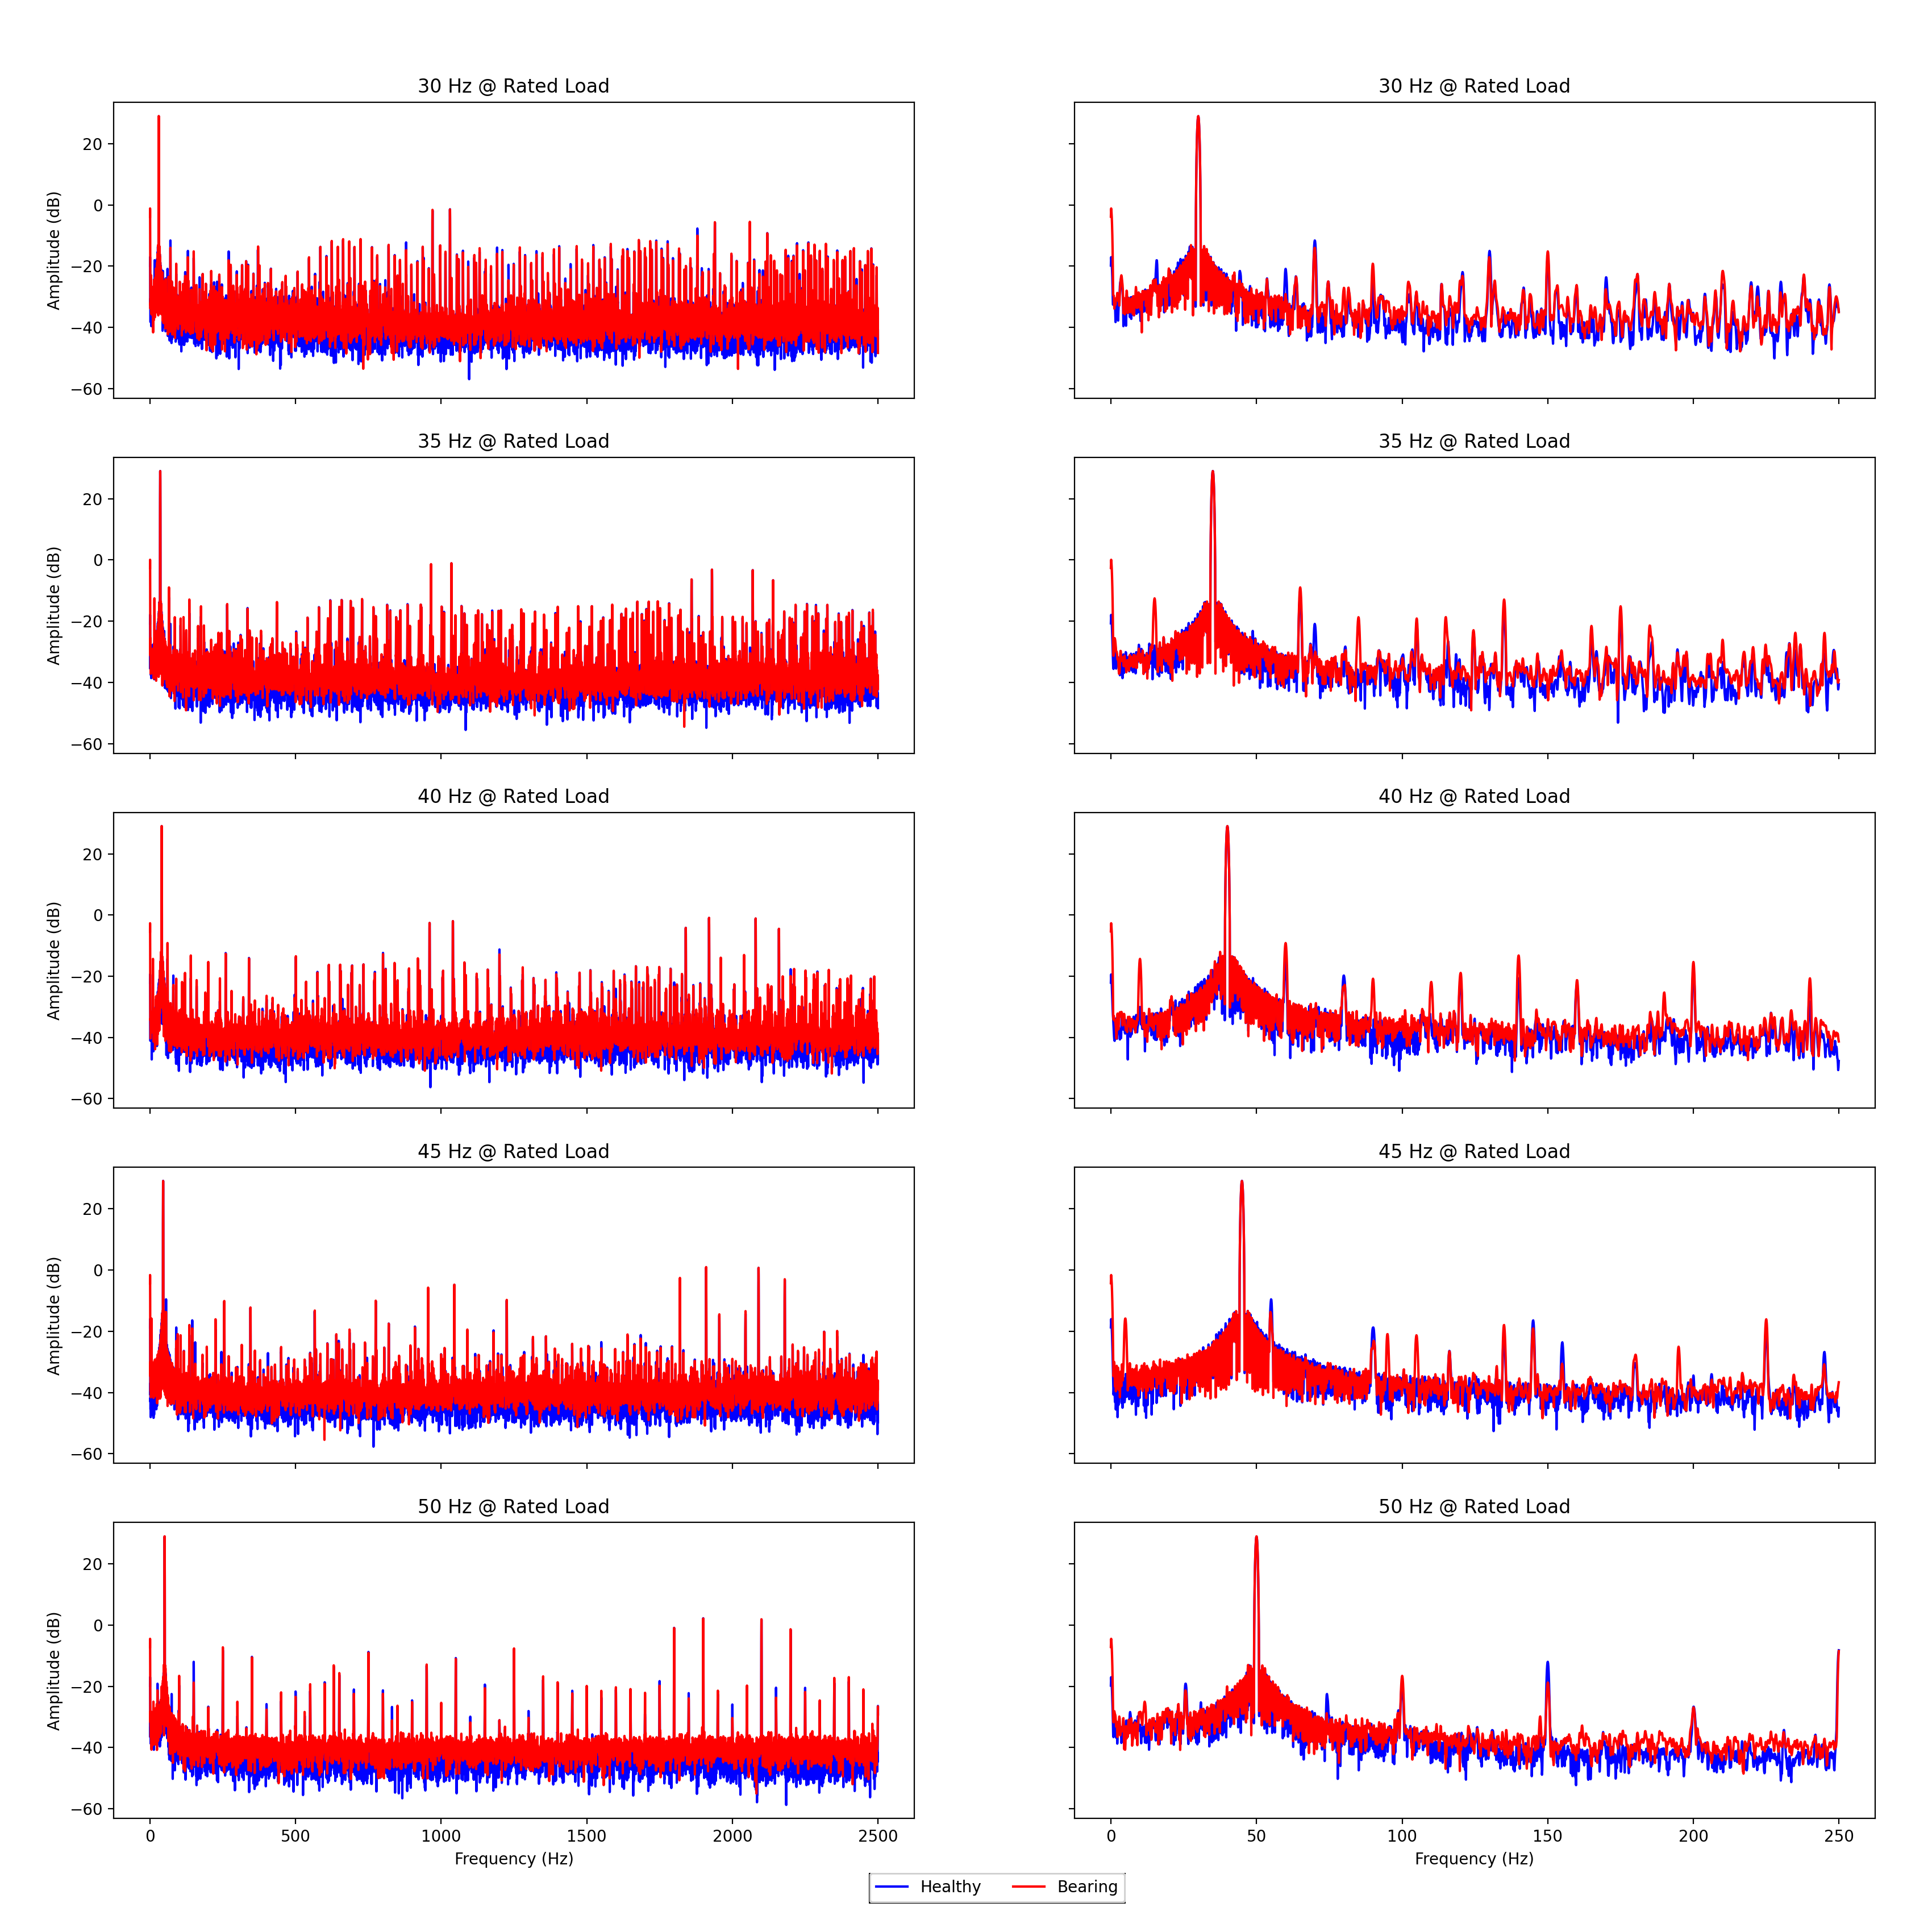
\includegraphics[width=0.8\paperwidth,keepaspectratio=true]{./fig/psdbearing_100.png}
	% sekil3.eps: 0x0 pixel, 300dpi, 0.00x0.00 cm, bb=14 14 1155 740
	\caption{Welch's PSD estimations of healthy and bearing-fault motor at rated load.}	
	\label{psdbearing100}
\end{figure}
\pagebreak
\begin{figure}[h]
	\centering
	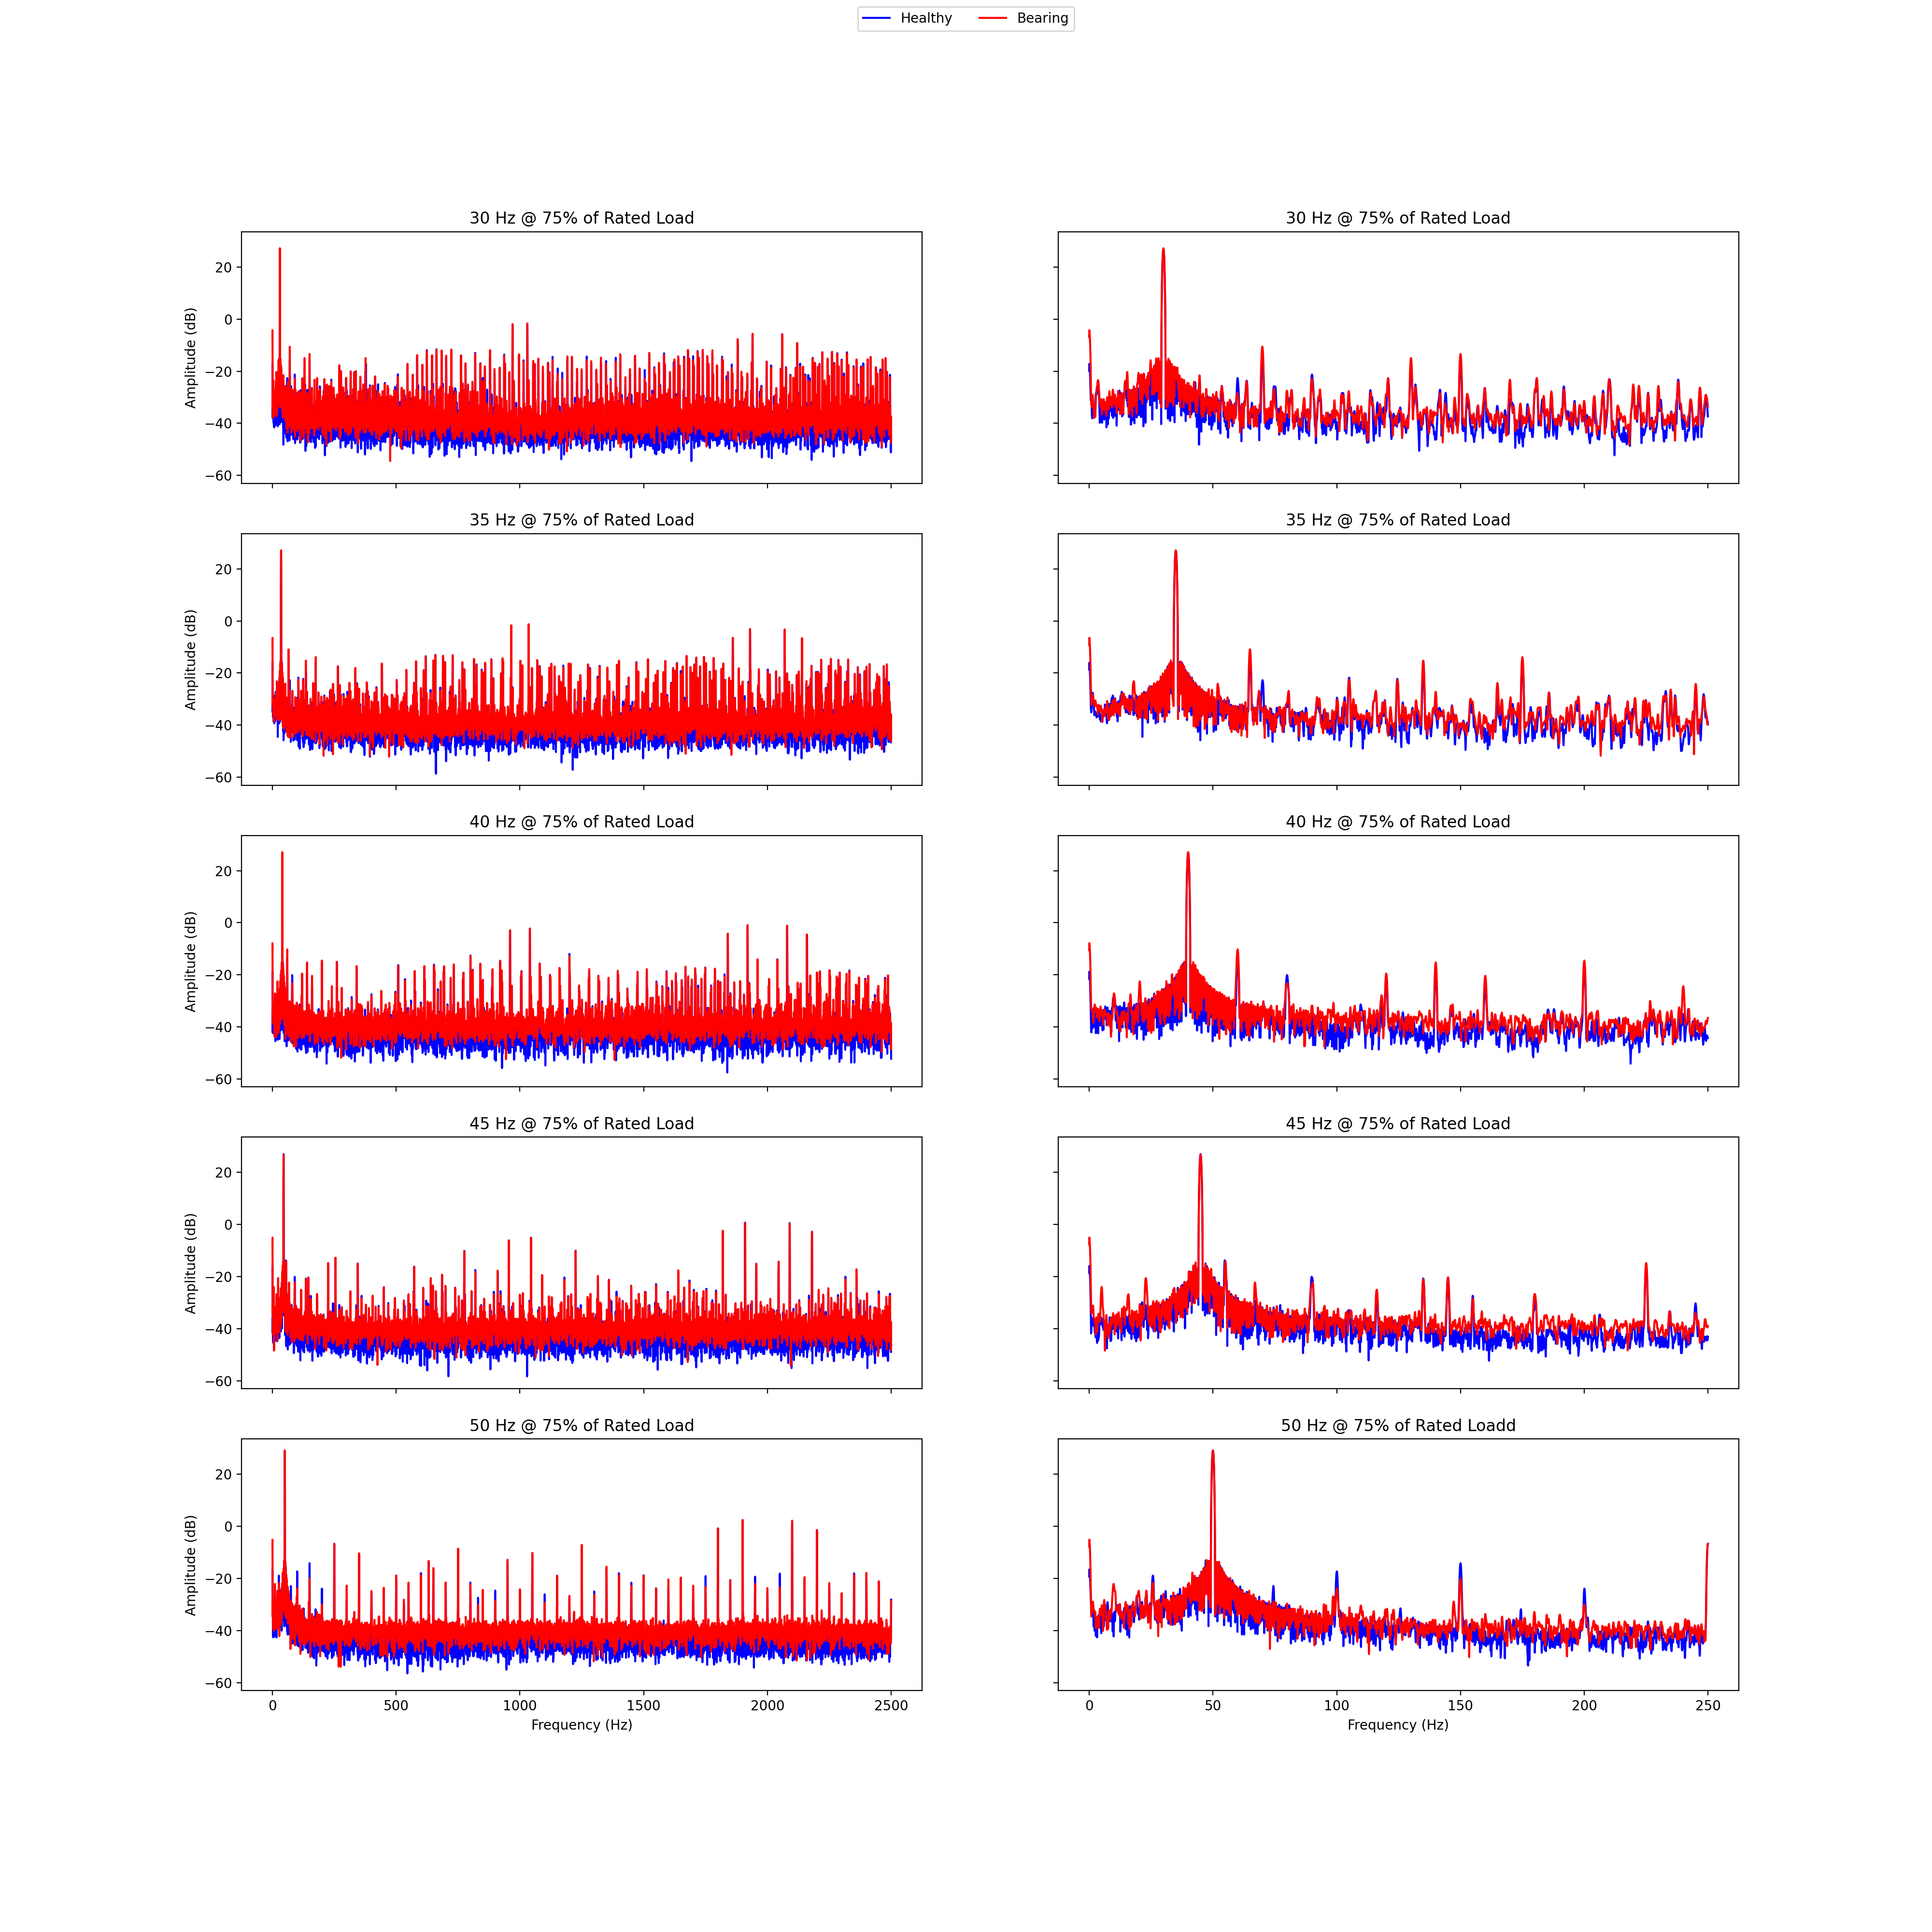
\includegraphics[width=0.8\paperwidth,keepaspectratio=true]{./fig/psdbearing_75.png}
	% sekil3.eps: 0x0 pixel, 300dpi, 0.00x0.00 cm, bb=14 14 1155 740
	\caption{Welch's PSD estimations of healthy and bearing-fault motor at $75\%$ of the rated load.}	
	\label{psdbearing75}
\end{figure}
\pagebreak
\begin{figure}[h]
	\centering
	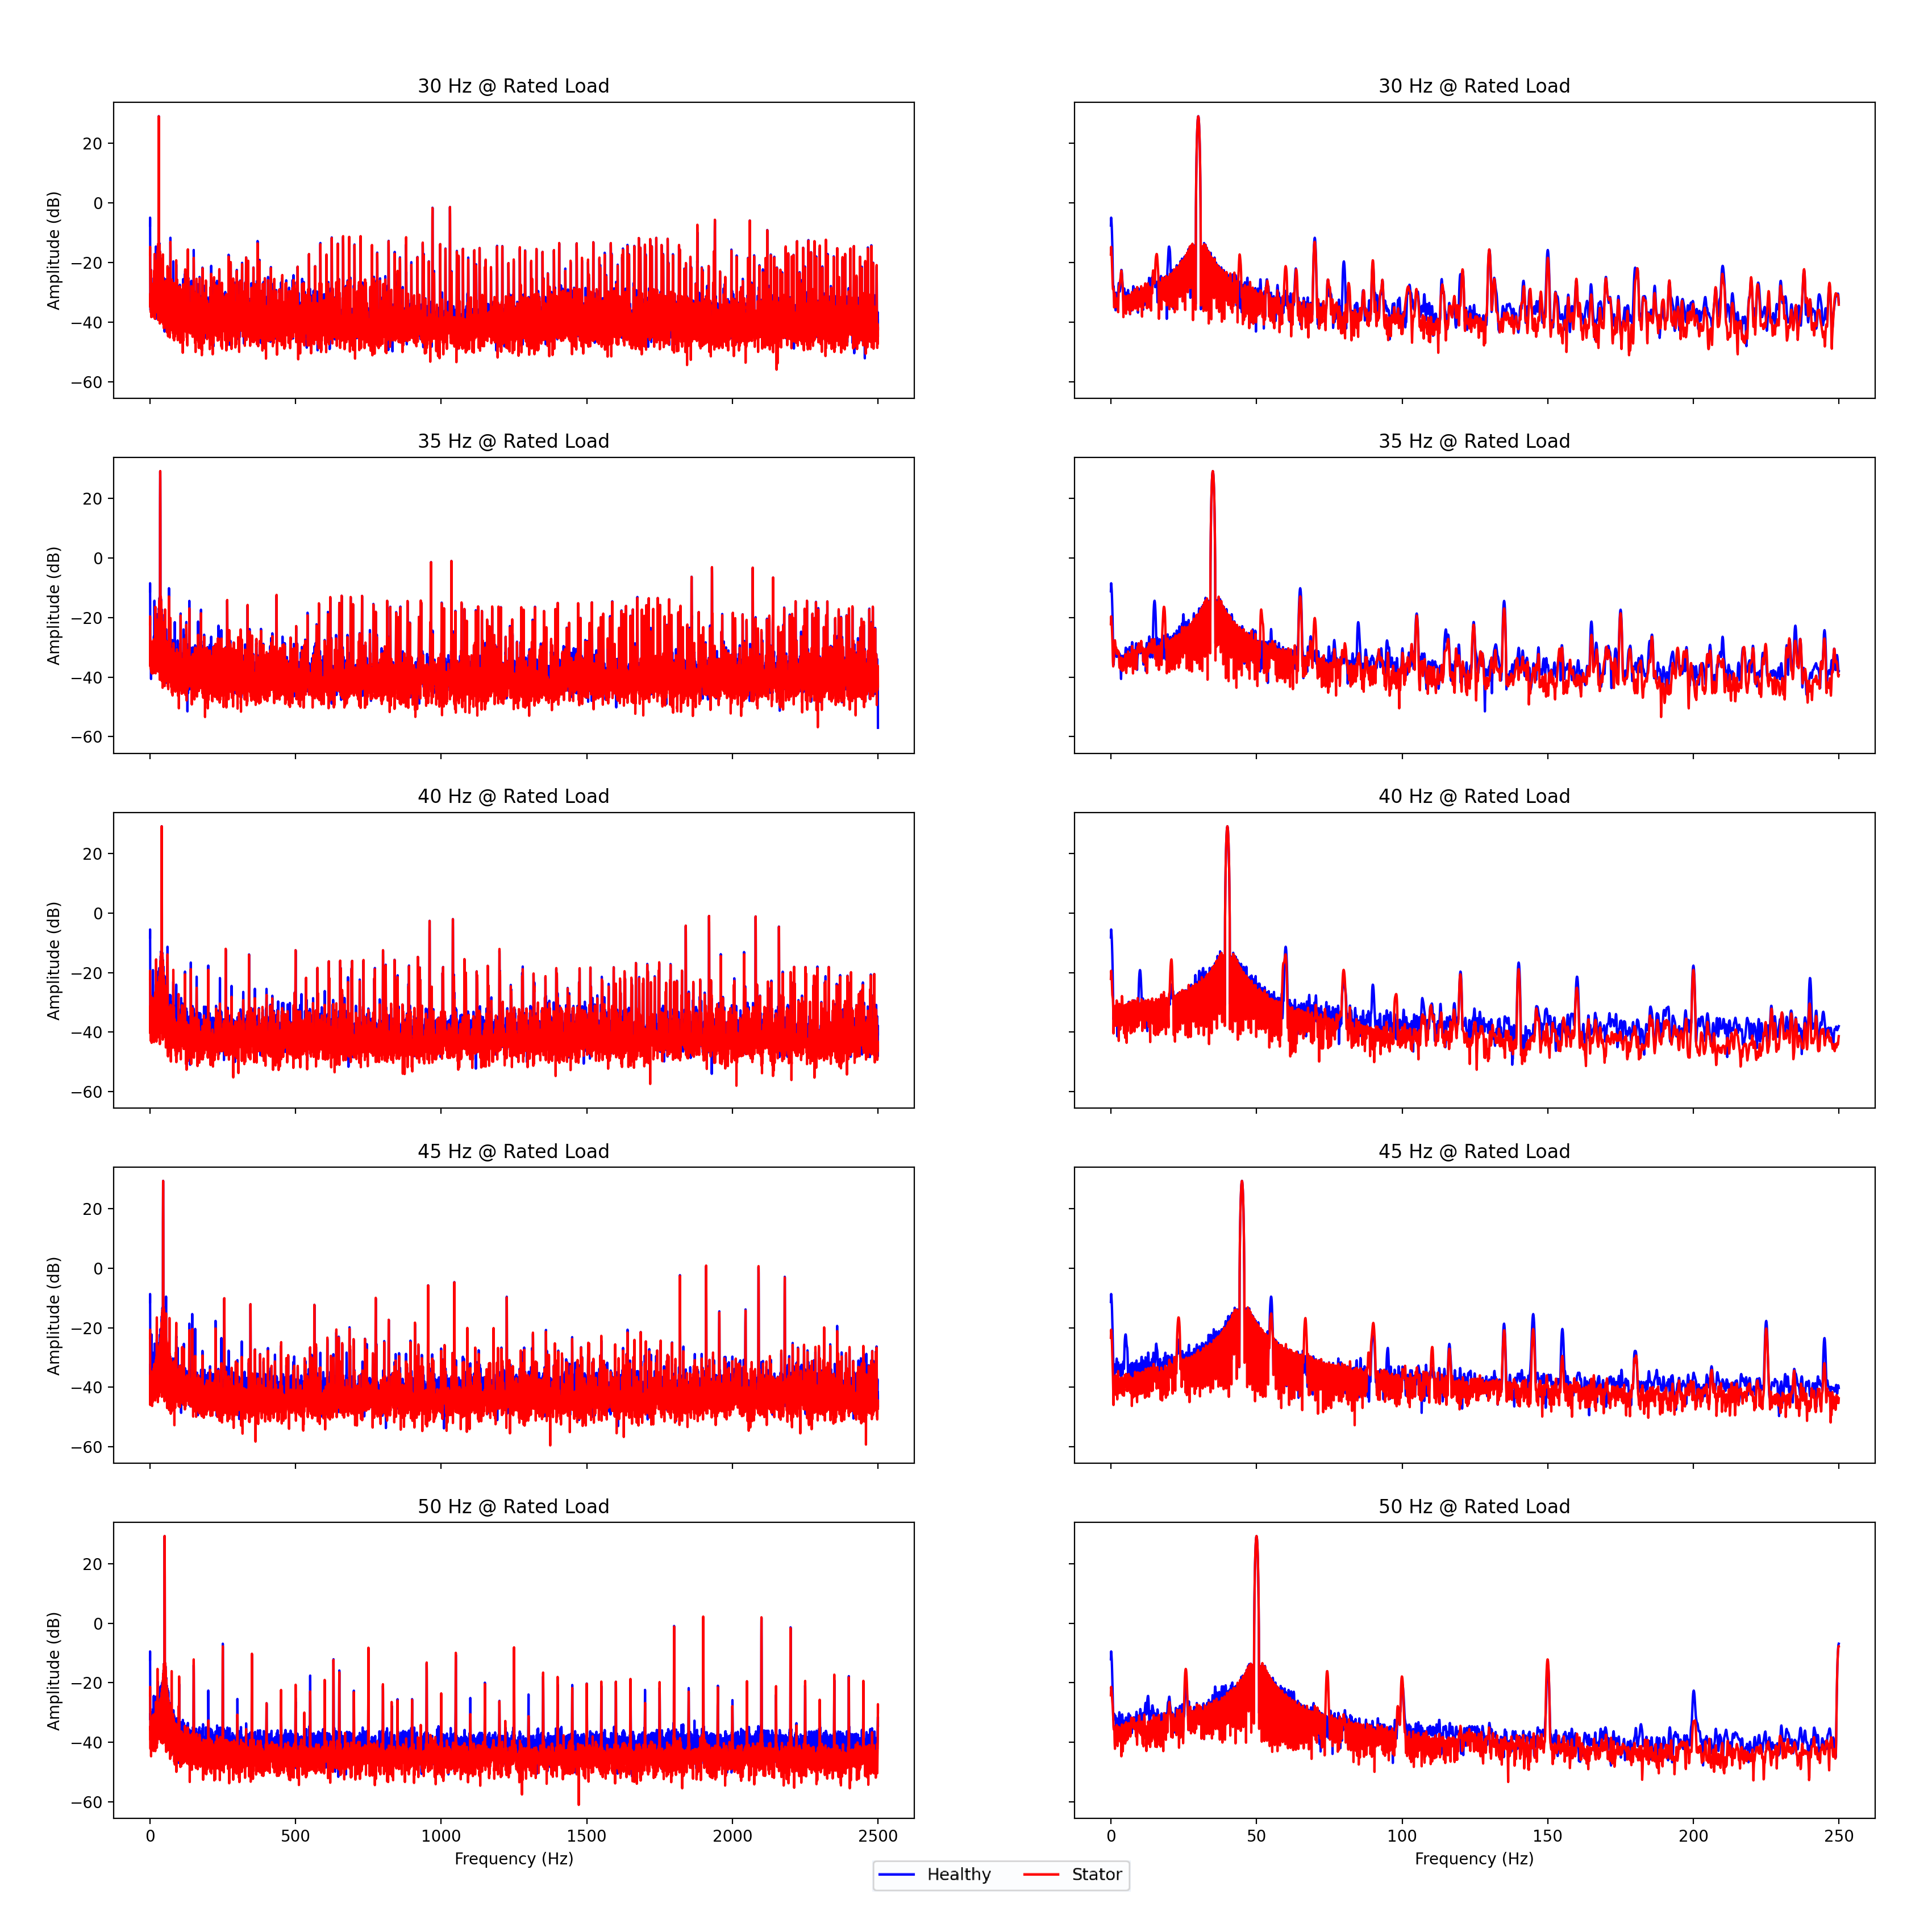
\includegraphics[width=0.8\paperwidth,keepaspectratio=true]{./fig/psdstator_100.png}
	% sekil3.eps: 0x0 pixel, 300dpi, 0.00x0.00 cm, bb=14 14 1155 740
	\caption{Welch's PSD estimations of healthy and Stator inter-turn-fault motor at 75$\%$ of the rated load.}	
	\label{psdstator100}
\end{figure}
\pagebreak
\begin{figure}[h]
	\centering
	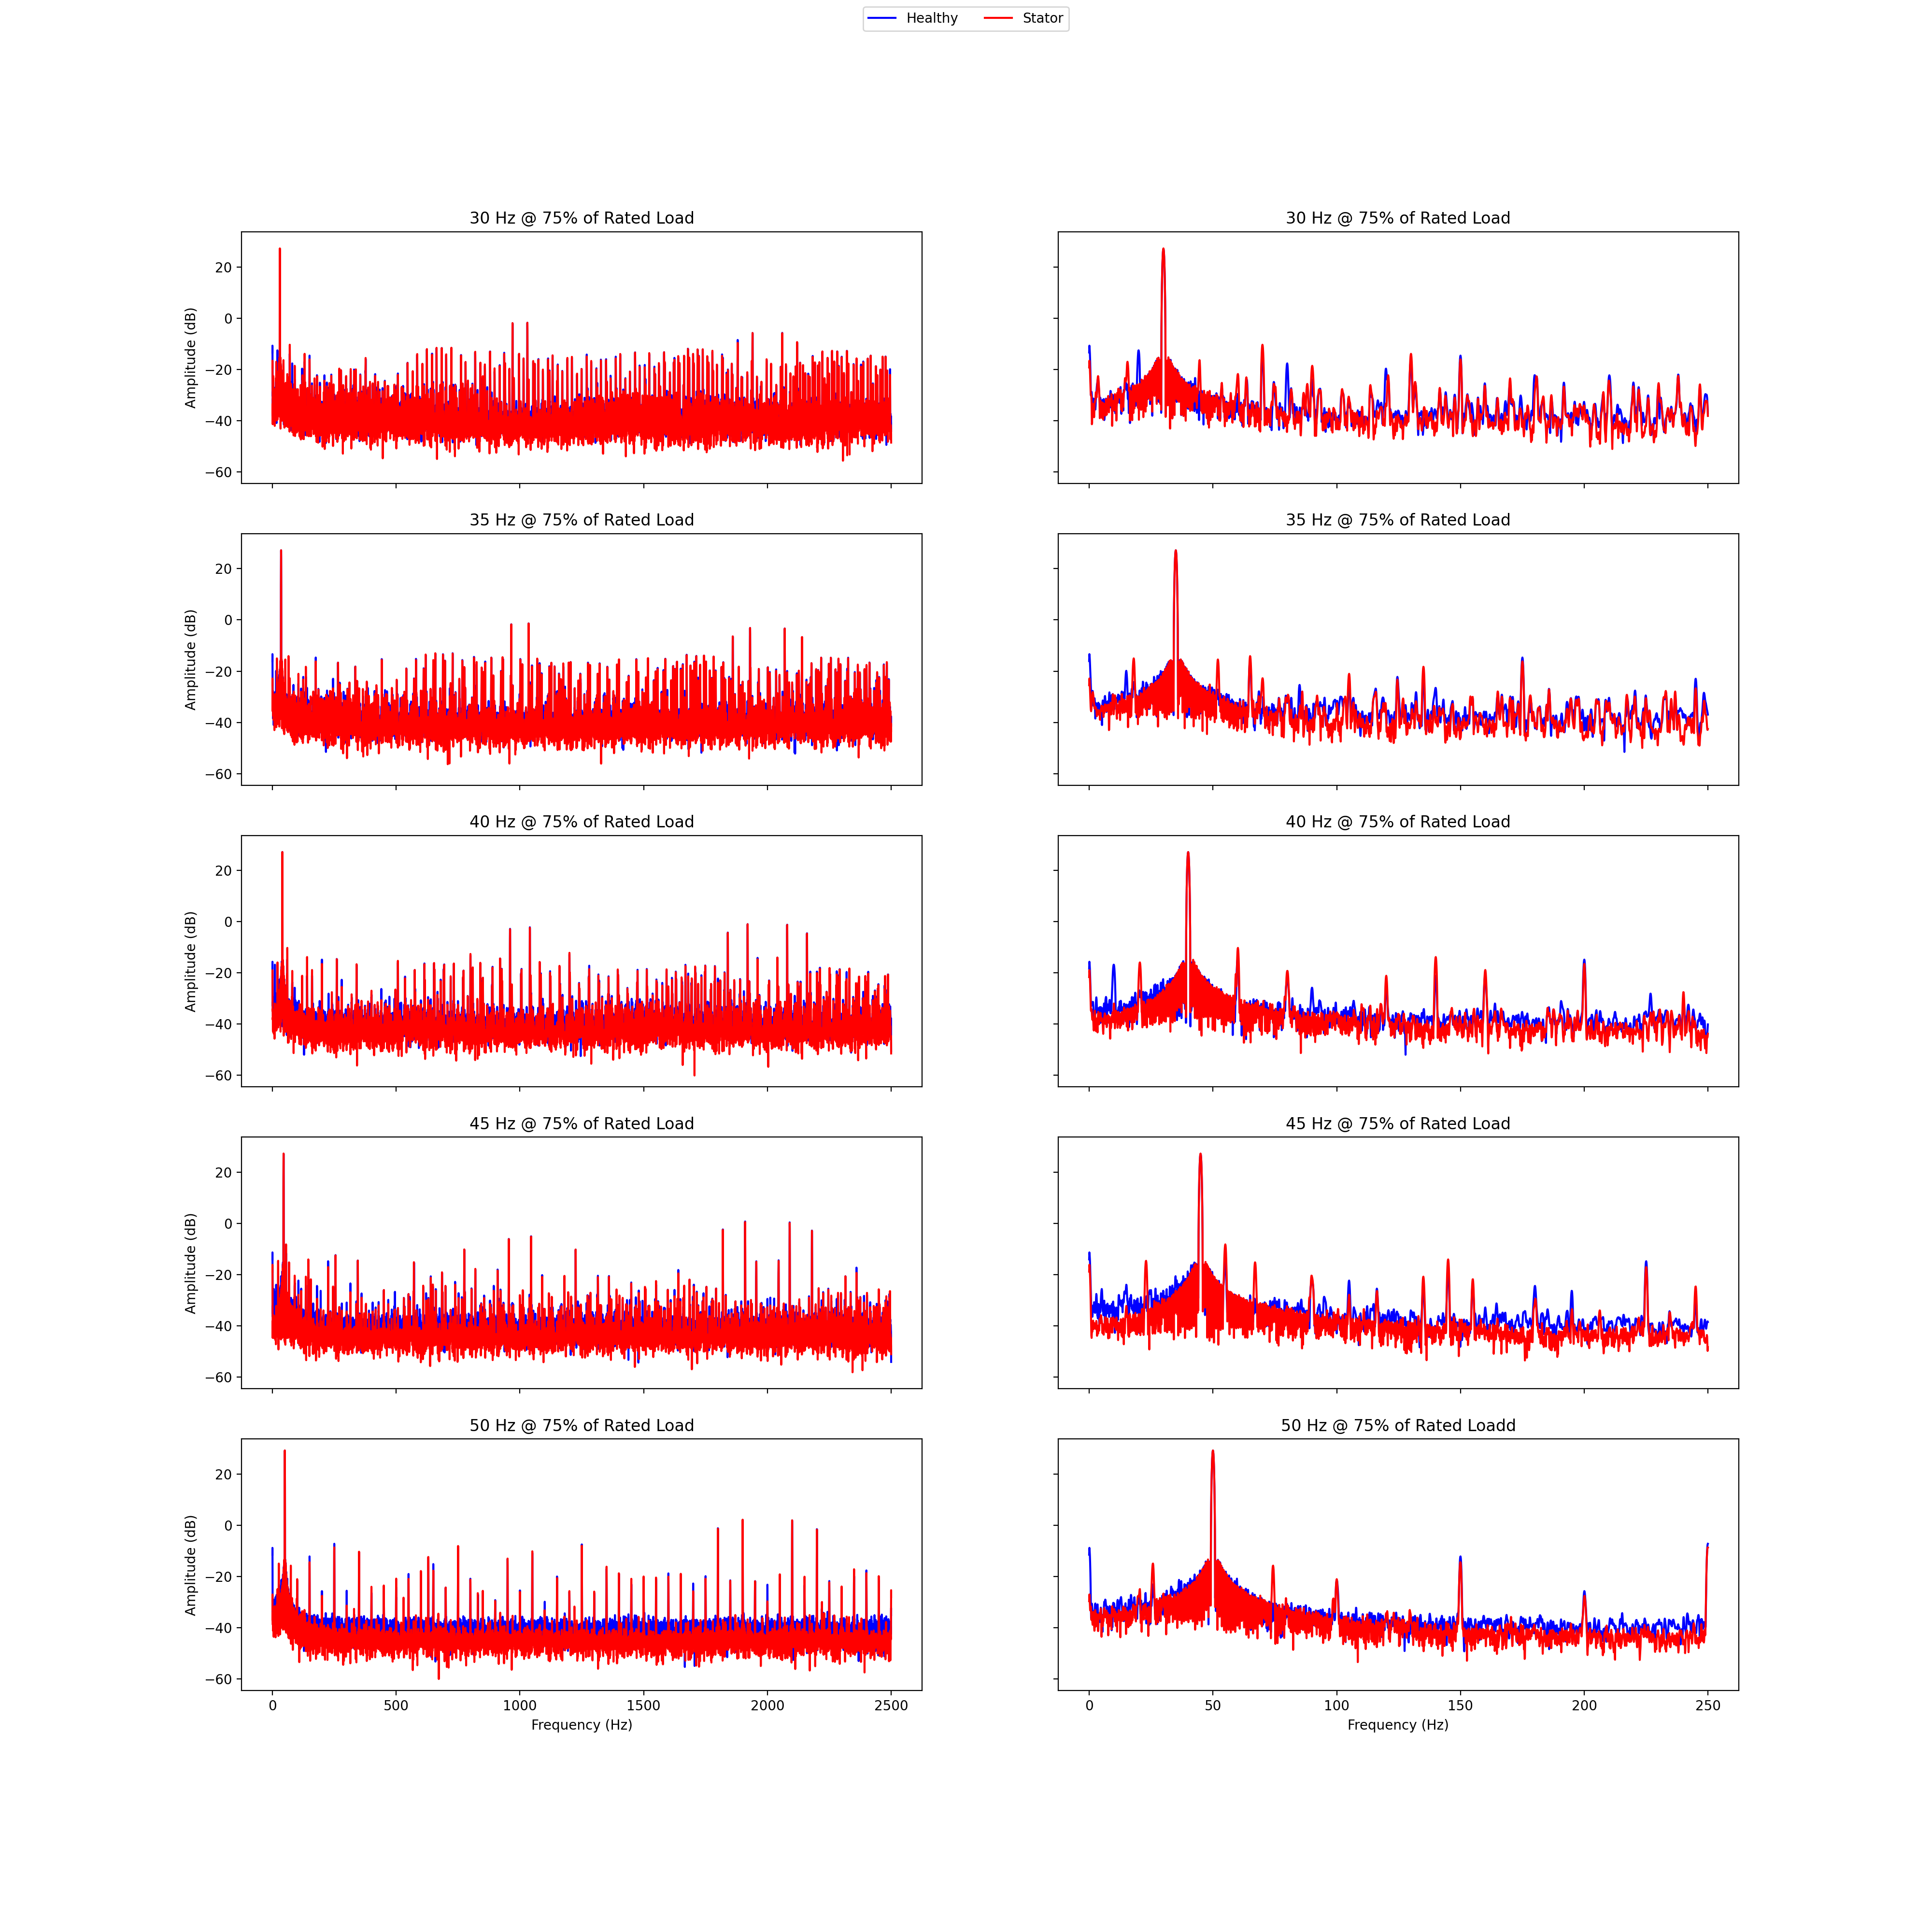
\includegraphics[width=0.8\paperwidth,keepaspectratio=true]{./fig/psdstator_75.png}
	% sekil3.eps: 0x0 pixel, 300dpi, 0.00x0.00 cm, bb=14 14 1155 740
	\caption{Welch's PSD estimations of healthy and Stator inter-turn-fault motor at 75$\%$ of the rated load.}	
	\label{psdstator75}
\end{figure}
\pagebreak
\begin{figure}[h]
	\centering
	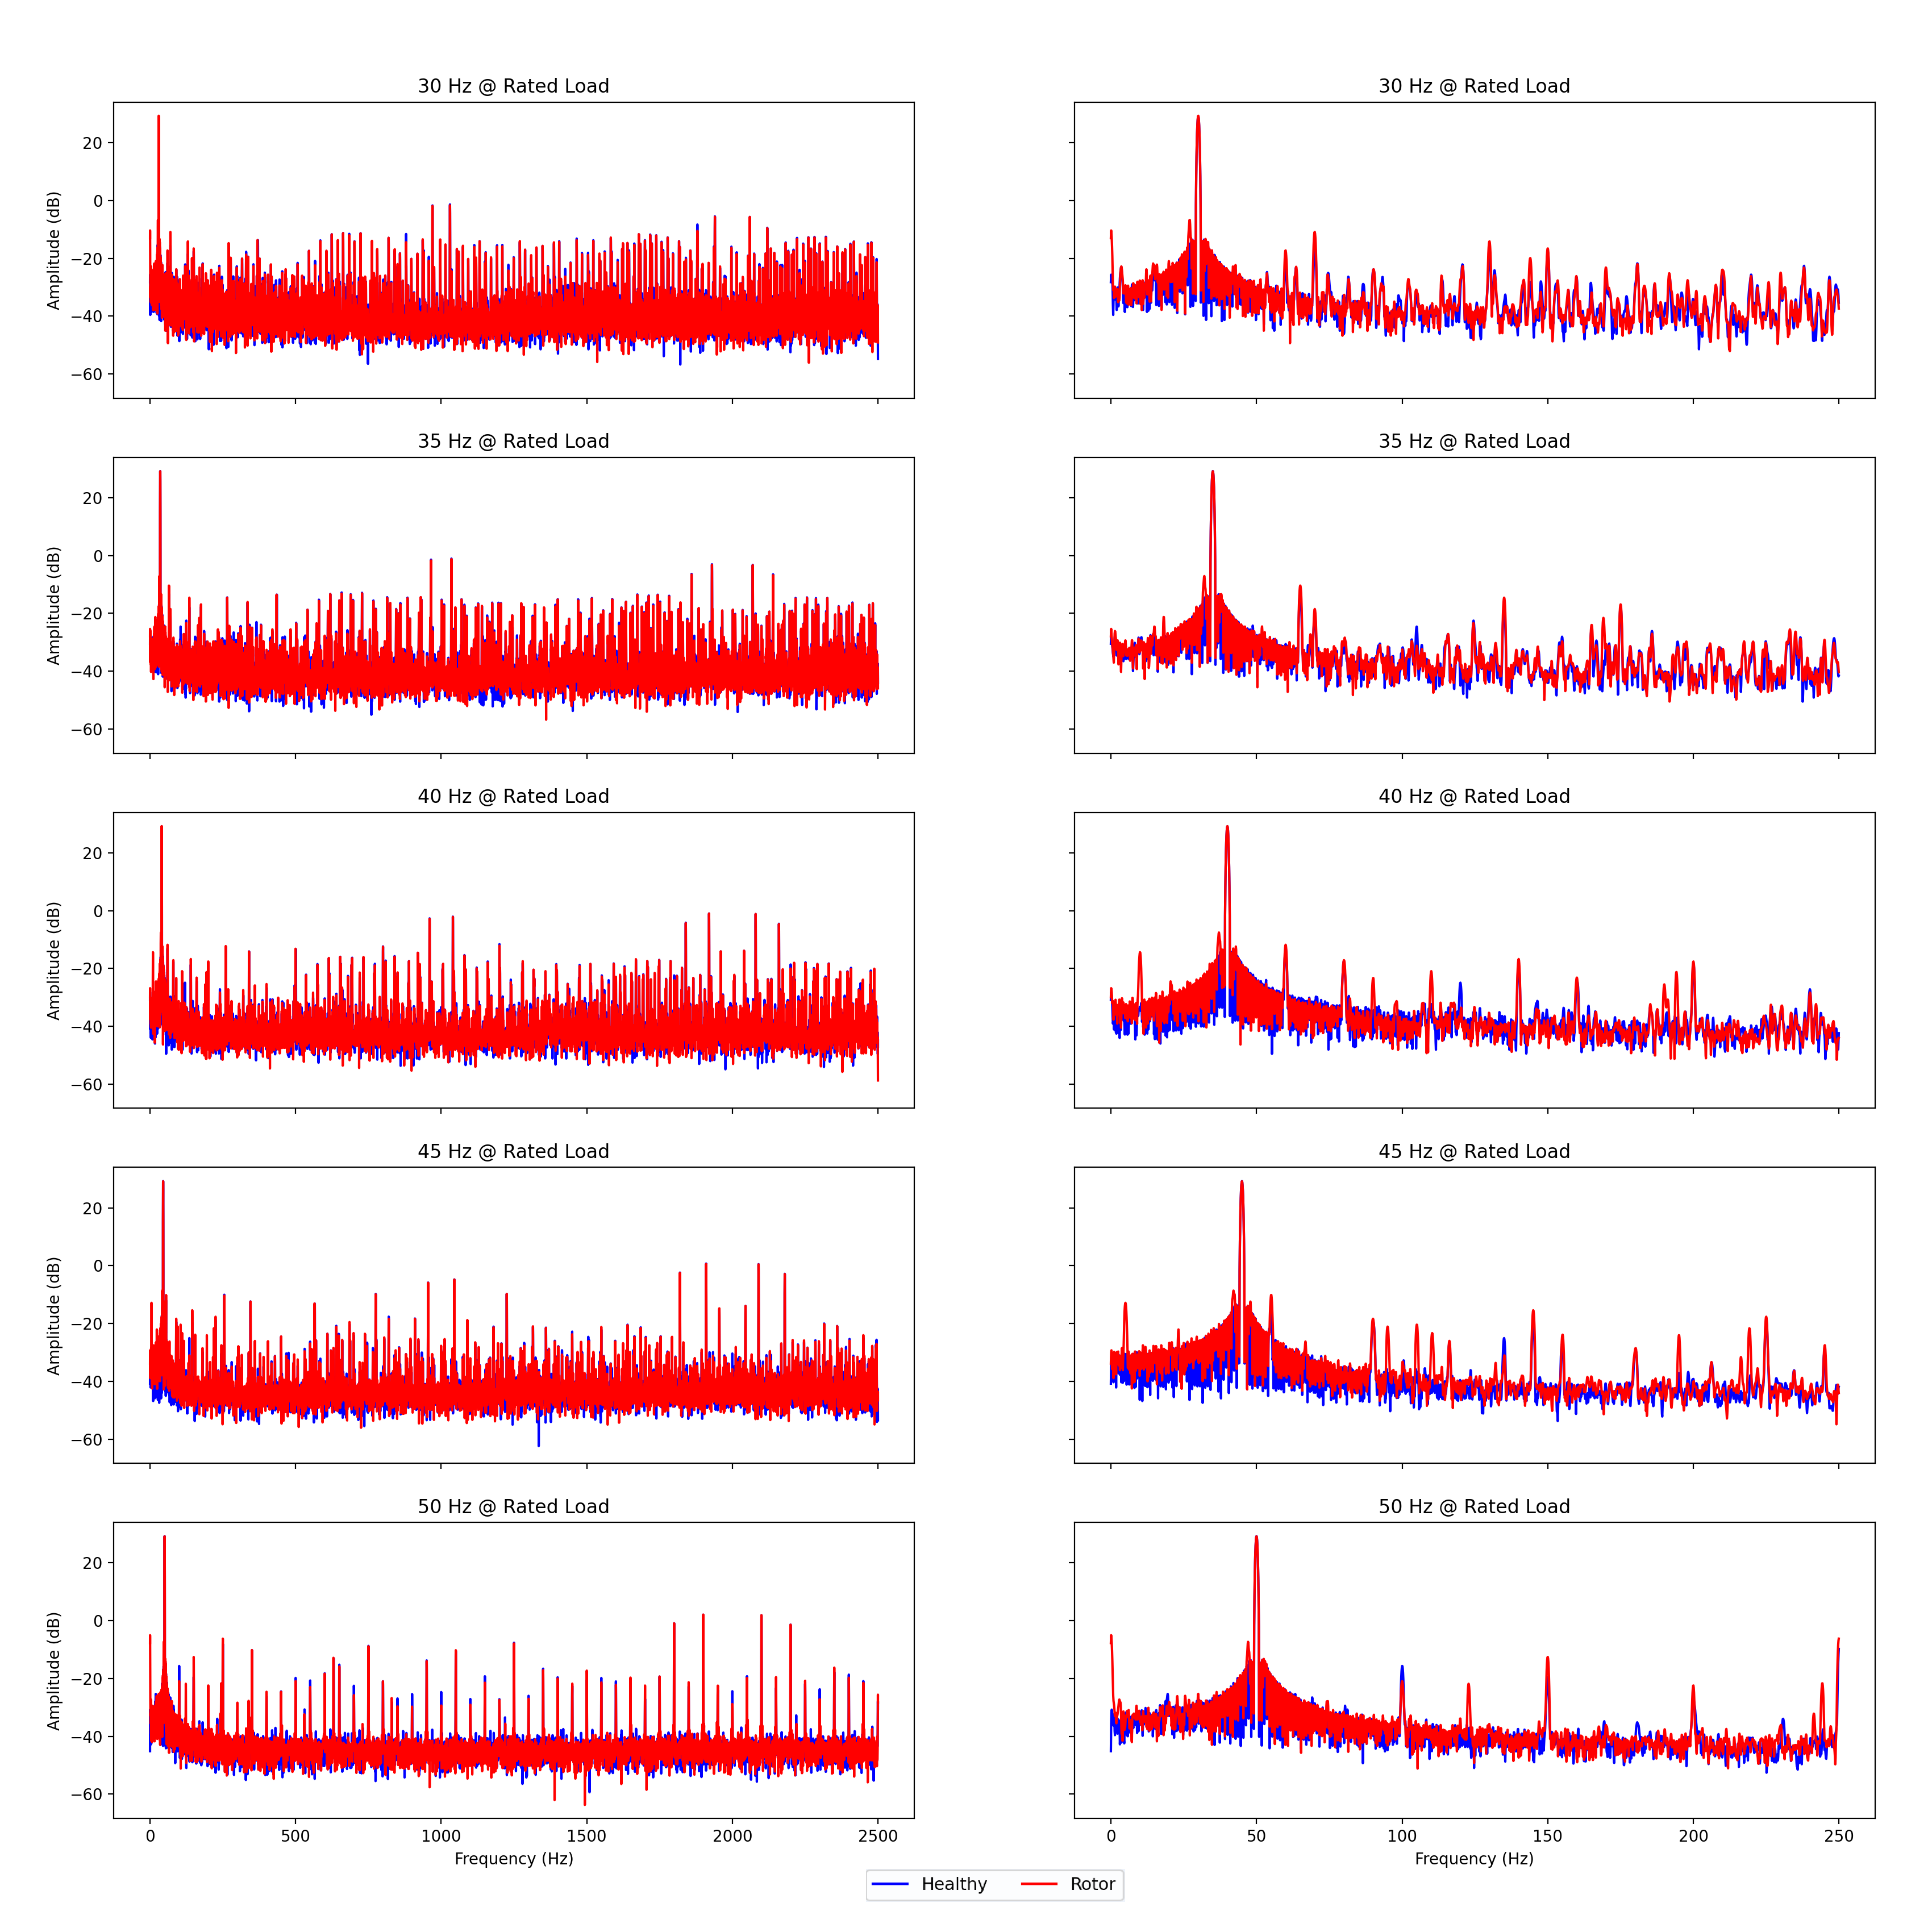
\includegraphics[width=0.8\paperwidth,keepaspectratio=true]{./fig/psdrotor_100.png}
	% sekil3.eps: 0x0 pixel, 300dpi, 0.00x0.00 cm, bb=14 14 1155 740
	\caption{Welch's PSD estimations of healthy and 1-Bar Broken Rotor-fault motor at 75$\%$ of the rated load.}	
	\label{psdrotor100}
\end{figure}
\pagebreak
\begin{figure}[h]
	\centering
	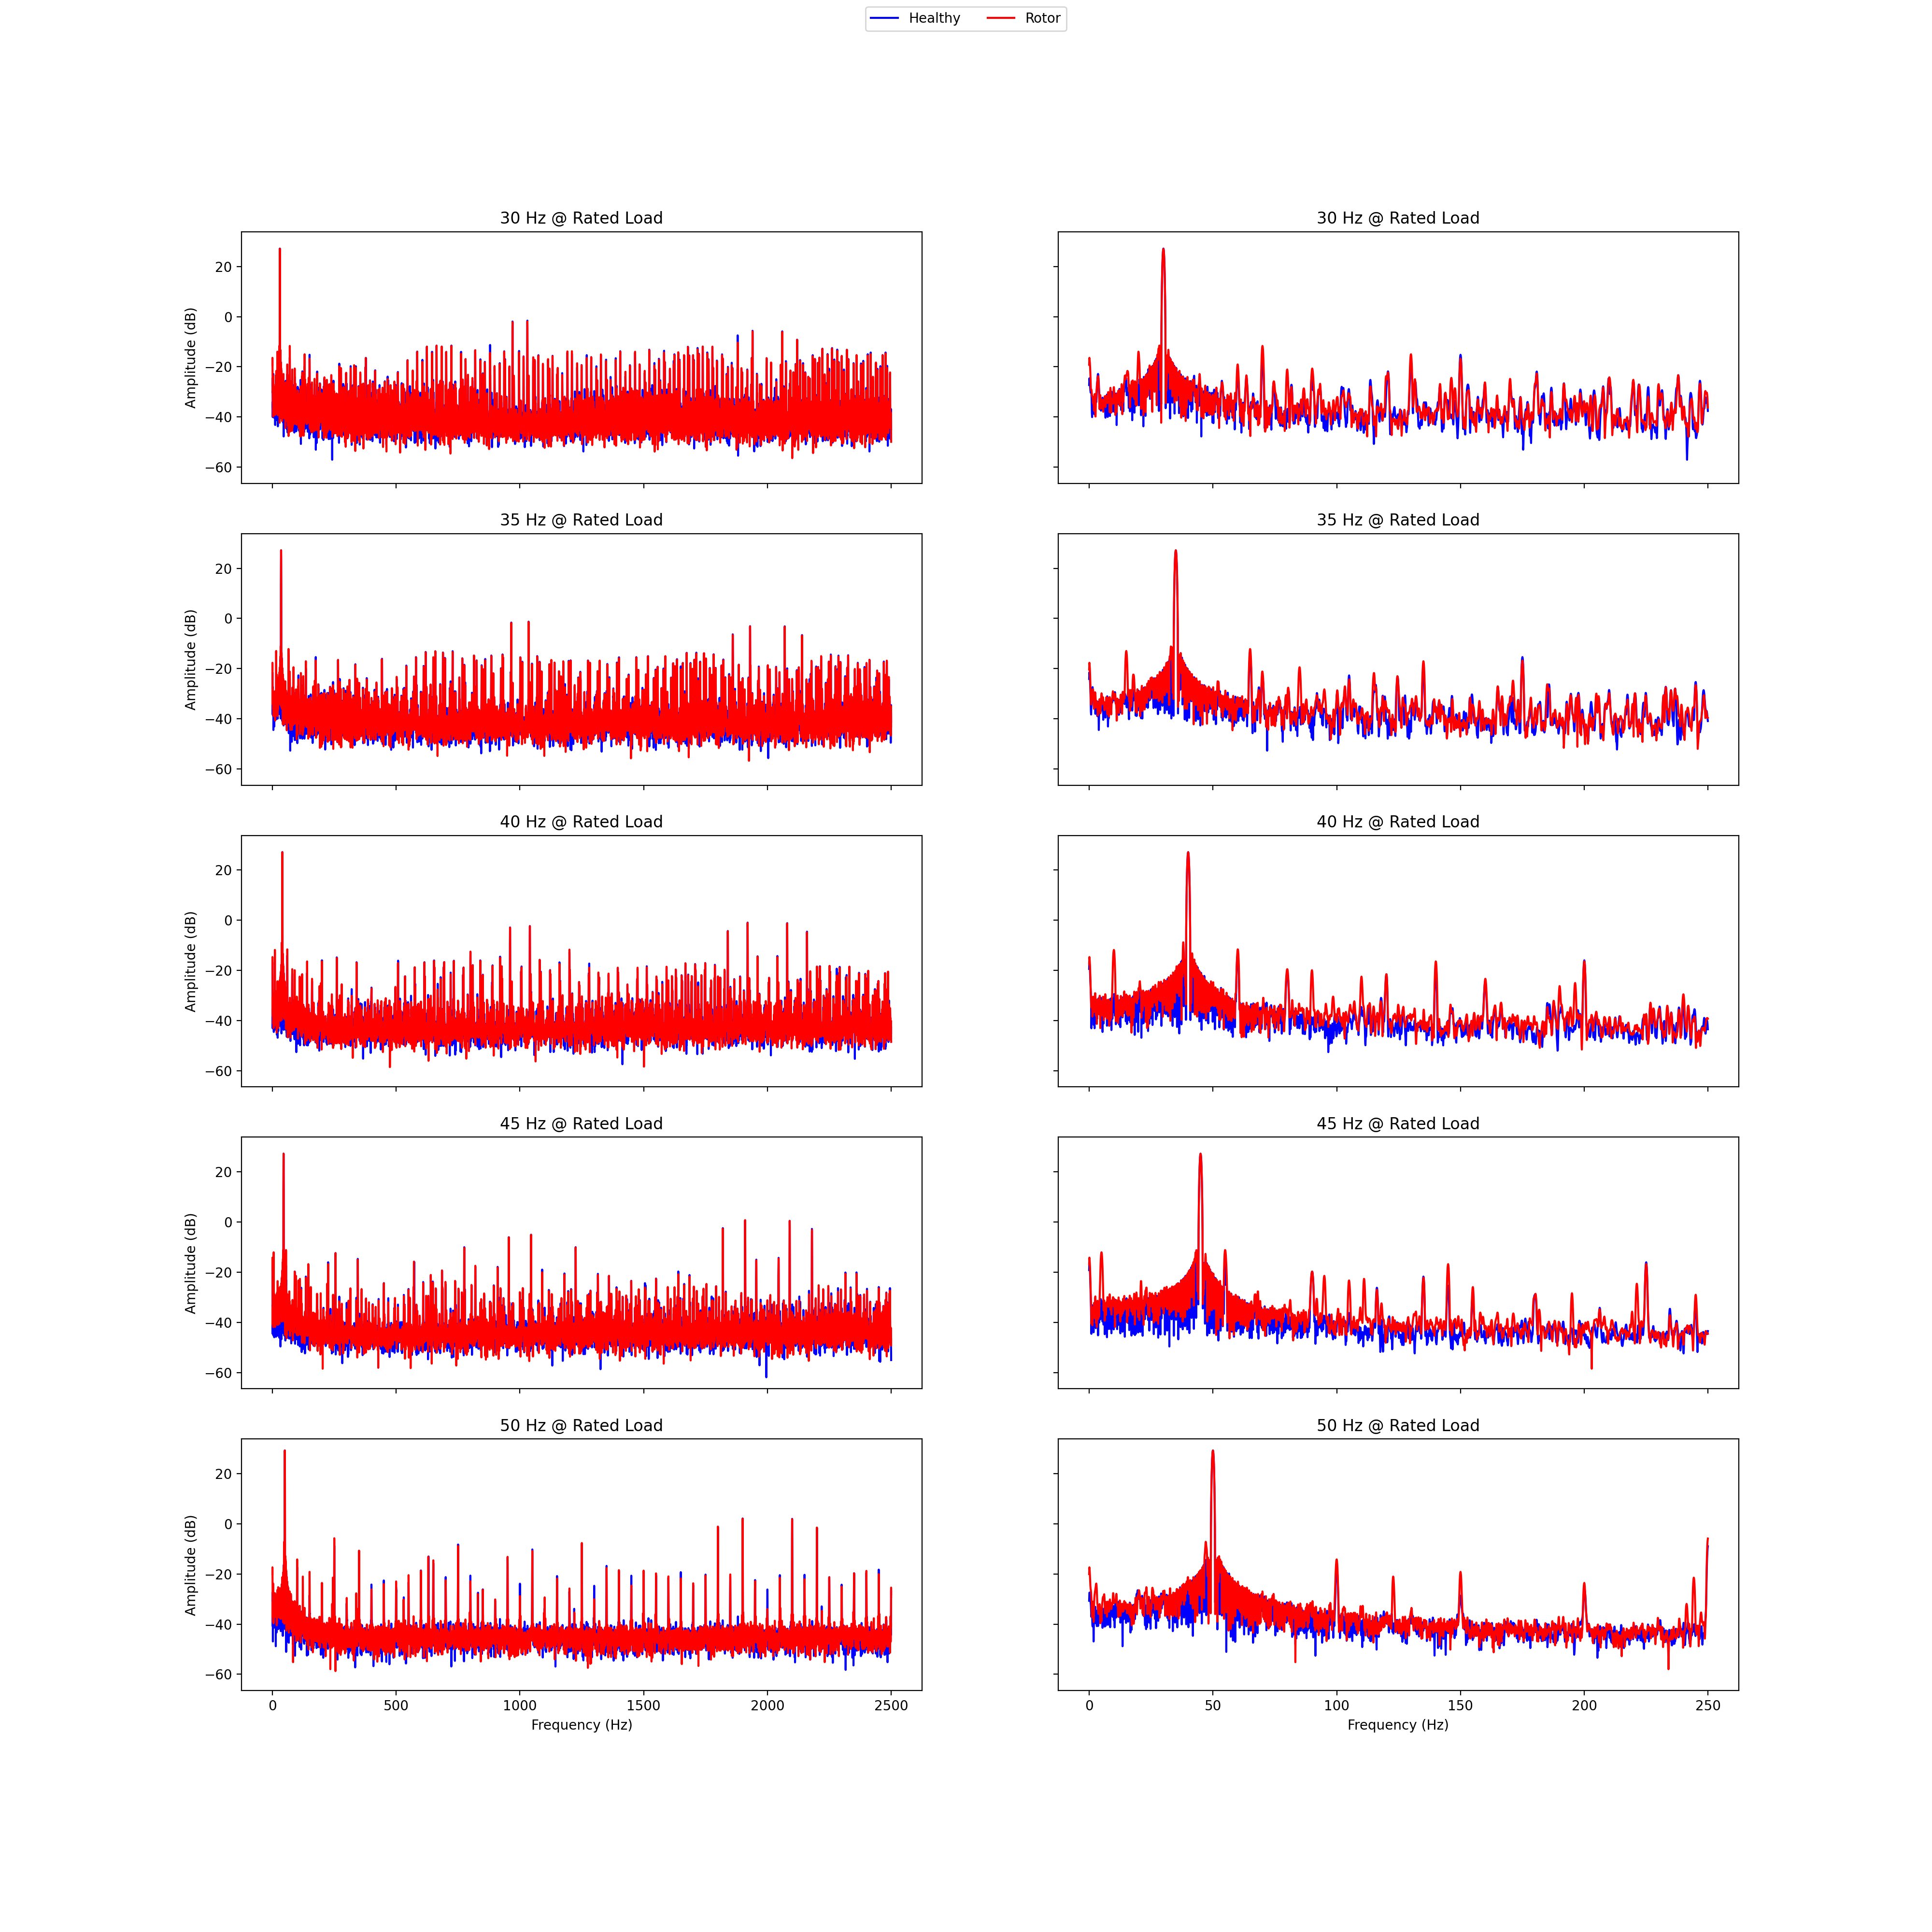
\includegraphics[width=0.8\paperwidth,keepaspectratio=true]{./fig/psdrotor_75.png}
	% sekil3.eps: 0x0 pixel, 300dpi, 0.00x0.00 cm, bb=14 14 1155 740
	\caption{Welch's PSD estimations of healthy and 1-Bar Broken Rotor-fault motor at 75$\%$ of the rated load.}
	\label{psdrotor75}
\end{figure}

% Lorem ipsum dolor sit amet, consetetur sadipscing elitr, sed diam nonumy eirmod tempor invidunt ut labore et dolore magna aliquyam erat, sed diam voluptua. At vero eos et accusam et justo duo dolores et ea rebum. Stet clita kasd gub rgren, no sea takimata sanctus est Lorem ipsum dolor sit amet, consetetur sadipscing elitr, sed diam nonumy eirmod tempor invidunt ut lab ore sit et dolore magna.

% Lorem ipsum dolor sit amet, consetetur sadipscing elitr, sed diam nonumy eirmod tempor invidunt ut labore et dolore magna aliquyam erat, sed diam voluptua. At vero eos et accusam et justo duo dolores et ea rebum. Stet clita kasd gub rgren, no sea takimata sanctus est Lorem ipsum dolor sit amet, consetetur sadipscing elitr, sed diam nonumy eirmod tempor invidunt ut lab ore sit et dolore magna.
 
% %\subsection{Page Margins}

% Lorem ipsum dolor sit amet, consetetur sadipscing elitr, sed diam Lorem ipsum dolor sit amet, consetetur sadipscing elitr, sed diam nonumy eirmod tempor invidunt ut labore et dolore magna aliquyam erat, sed diam voluptua. At vero eos et accusam et justo duo dolores et ea rebum (Figure \ref{Figure3.1}).

% The gap at the bottom of the page is 2.5 cm. 

% Keeping more redundant space is incorrect. So, this gap should not be. Texts, tables, figures, etc. in the pages must be arranged considering this situation.

% %\setitemize{leftmargin=2em} % Left margin given to the bullets - SBÖ
% \begin{itemize}
% 	\setlength{\itemindent}{-0.35em} % Flush the bullets to the left - SBÖ
% 	\item{Figures, tables can be enlarged and be reduced.}
% 	\vspace{-3mm}
% 	\item{The explanations except from the first reference about the figure or table can be placed either before the figure/table or after.}
% 	\vspace{-3mm}
% 	\item{After referring to a figure or table it is placed to the closest and convenient location. Convenient location must be arranged considering the gap at the bottom of the page.}
% \end{itemize}

% \begin{figure}
% %\begin{sidewaysfigure}
% 	\centering
% 	
\includegraphics[width=280pt,keepaspectratio=true]{./fig/sekil3}
% 	% sekil3.eps: 0x0 pixel, 300dpi, 0.00x0.00 cm, bb=14 14 1155 740
% 	\caption{Neuron cell, adapted from (\c{C}etin, 2003).}
% 	\label{Figure3.1}
% %\end{sidewaysfigure}
% \end{figure}

% Lorem ipsum dolor sit amet, consetetur sadipscing elitr, sed diam nonumy eirmod tempor invidunt ut labore et dolore magna aliquyam erat, sed diam voluptua. At vero eos et accusam et justo duo dolores et ea rebum. Stet clita kasd gub rgren, no sea takimata sanctus est Lorem ipsum dolor sit amet, consetetur sadipscing elitr, sed diam nonumy eirmod tempor invidunt ut lab ore sit et dolore magna.

% At vero eos et accusam et justo duo dolores et ea rebum. Stet clita kasd gub rgren, no sea takimata sanctus est Lorem ipsum dolor sit amet, consetetur sadipscing elitr, sed diam nonumy eirmod tempor invidunt ut lab ore sit et dolore magna.

% Lorem ipsum dolor sit amet, consetetur sadipscing elitr, sed diam nonumy eirmod tempor invidunt ut labore et dolore magna aliquyam erat, sed diam voluptua. At vero eos et accusam et justo duo dolores et ea rebum. Stet clita kasd gub rgren, no sea takimata sanctus est Lorem ipsum dolor sit amet, consetetur sadipscing elitr, sed diam nonumy eirmod tempor invidunt ut lab ore sit et dolore magna.

% %\subsection{Equations}

% Lorem ipsum dolor sit amet, consetetur sadipscing elitr, sed diam nonumy eirmod tempor invidunt ut labore et dolore magna aliquyam erat, sed diam voluptua. At vero eos et accusam et justo duo dolores et ea rebum. Stet clita kasd gub rgren, no sea takimata sanctus est  Lorem ipsum dolor sit amet, consetetur sadipscing elitr, sed diam nonumy eirmod tempor invidunt ut lab  ore sit et dolore magna equation (\ref{Eq3.1}).
% \begin{equation}
% y_{t} = \phi_{1} y_{t-1} + \epsilon_{t}
% \label{Eq3.1}
% \end{equation}
% Lorem ipsum dolor sit amet, consetetur sadipscing elitr, sed diam nonumy eirmod tempor invidunt ut labore et dolore magna aliquyam erat, sed diam voluptua. At vero eos et accusam et justo duo dolores et ea rebum. Stet clita kasd gub rgren, no sea takimata sanctus est Lorem ipsum dolor sit amet, consetetur sadipscing elitr, sed diam nonumy eirmod tempor invidunt ut lab ore sit et dolore magna.
% % Subequation example - SBÖ
% \vskip -24pt
% \begin{subequations}
% 	\begin{gather}
% 	R_0 = 0 \label{Eq3.2a}\\
% 	N_0 = 0 \label{Eq3.2b}
% 	\end{gather}
% 	\label{Eq3.2ab}
% \end{subequations}
% \vskip -24pt
% Each parameter is described, as seen in equation \eqref{Eq3.1}, or in \ref{Eq3.1}. Lorem ipsum dolor sit amet, consetetur sadipscing elitr, sed diam nonumy eirmod tempor invidunt ut labore et dolore equation \ref{Eq3.1}’in magna aliquyam erat Equation \eqref{Eq3.2ab} into Equation \eqref{Eq3.2a} and Equation \eqref{Eq3.2b}.

% %\subsection{Process based model: SWAT}

% Lorem ipsum dolor sit amet, consetetur sadipscing elitr, sed diam nonumy eirmod tempor invidunt ut labore et dolore magna aliquyam erat, sed diam voluptua. At vero eos et accusam et justo duo dolores et ea rebum. Stet clita kasd gub rgren, no sea takimata sanctus est Lorem ipsum dolor sit amet, consetetur sadipscing elitr, sed diam nonumy eirmod tempor invidunt ut lab ore sit et dolore magna.

% Lorem ipsum dolor sit amet, consetetur sadipscing elitr, sed diam nonumy eirmod tempor invidunt ut labore et dolore magna aliquyam erat, sed diam voluptua. At vero eos et accusam et justo duo dolores et ea rebum. Stet clita kasd gub rgren, no sea takimata sanctus est Lorem ipsum dolor sit amet, consetetur sadipscing elitr, sed diam nonumy eirmod tempor invidunt ut lab ore sit et dolore magna.

% \begin{figure}
% 	\centering
% 	
\includegraphics[width=250pt,keepaspectratio=true]{./fig/sekil3}
% 	% sekil3.eps: 0x0 pixel, 300dpi, 0.00x0.00 cm, bb=14 14 1155 740
% 	\caption{For a multi-line figure captions, it is important that all the lines of the caption are aligned.}
% 	\label{Figure3.2}
% \end{figure}

% %\subsection{Multi variable analysis}

% Lorem ipsum dolor sit amet, consetetur sadipscing elitr, sed diam nonumy eirmod tempor invidunt ut labore et dolore magna aliquyam erat, sed diam voluptua. At vero eos et accusam et justo duo dolores et ea rebum. Stet clita kasd gub rgren, no sea takimata sanctus est Lorem ipsum dolor sit amet, consetetur sadipscing elitr, sed diam nonumy eirmod tempor invidunt ut lab ore sit et dolore magna (\ref{Eq3.2}). Lorem ipsum dolor sit amet, consetetur sadipscing elitr, sed diam nonumy eirmod tempor invidunt ut labore et dolore magna aliquyam erat, sed diam voluptua. At vero eos et accusam et justo duo dolores et ea rebum. Lorem ipsum dolor sit amet, consetetur sadipscing elitr, sed diam nonumy eirmod tempor invidunt ut labore et dolore magna aliquyam erat, sed diam voluptua. At vero eos et accusam et justo duo dolores et ea rebum. Lorem ipsum dolor sit amet, consetetur sadipscing elitr, sed diam nonumy eirmod tempor invidunt ut labore et dolore magna aliquyam erat, sed diam voluptua. At vero eos et accusam et justo duo dolores et ea rebum.

% \begin{figure}
% 	\centering
% 	
\includegraphics[width=250pt,keepaspectratio=true]{./fig/sekil4}
% 	% sekil4.eps: 0x0 pixel, 300dpi, 0.00x0.00 cm, bb=14 14 1148 603
% 	\caption{Figure captions must be ended with a full stop.}
% 	\label{Figure3.4}
% \end{figure}

% Lorem ipsum dolor sit amet, consetetur sadipscing elitr, sed diam nonumy eirmod tempor invidunt ut labore et dolore magna aliquyam erat, sed diam voluptua. Lorem ipsum dolor sit amet, consetetur sadipscing elitr, sed diam nonumy eirmod tempor invidunt ut labore et dolore magna aliquyam erat, sed diam voluptua. At vero eos et accusam et justo duo dolores et ea rebum. 
% \begin{equation}
% D\left(C_{A},C_{B}\right) = \min X_{A}\in C_{A},X_{B}\in C_{B} 
% d\left(X_{A},X_{B}\right)
% \label{Eq3.2}
% \end{equation}
% Lorem ipsum dolor sit amet, consetetur sadipscing elitr, sed diam nonumy eirmod tempor invidunt ut labore et dolore magna aliquyam erat, sed diam voluptua. Lorem ipsum dolor sit amet, consetetur sadipscing elitr, sed diam nonumy eirmod tempor invidunt ut labore et dolore magna aliquyam erat, sed diam voluptua. At vero eos et accusam et justo duo dolores et ea rebum. 

% %\section{Practical Applications}

% Lorem ipsum dolor sit amet, consetetur sadipscing elitr, sed diam nonumy eirmod tempor invidunt ut labore et dolore magna aliquyam erat, sed diam voluptua. At vero eos et accusam et justo duo dolores et ea rebum. Stet clita kasd gub rgren, no sea takimata sanctus est Lorem ipsum dolor sit amet, consetetur sadipscing elitr, sed diam nonumy eirmod tempor invidunt ut lab ore sit et dolore magna.

% Lorem ipsum dolor sit amet, consetetur sadipscing elitr, sed diam nonumy eirmod tempor invidunt ut labore et dolore magna aliquyam erat, sed diam voluptua. At vero eos et accusam et justo duo dolores et ea rebum. Stet clita kasd gub rgren, no sea takimata sanctus est Lorem ipsum dolor sit amet, consetetur sadipscing elitr, sed diam nonumy eirmod tempor invidunt ut lab ore sit et dolore magna.

% %\section{Application Data}

% Lorem ipsum dolor sit amet, consetetur sadipscing elitr, sed diam nonumy eirmod tempor invidunt ut labore et dolore magna aliquyam erat, sed diam voluptua. At vero eos et accusam et justo duo dolores et ea rebum. Stet clita kasd gub rgren, no sea takimata sanctus est Lorem ipsum dolor sit amet, consetetur sadipscing elitr, sed diam nonumy eirmod tempor invidunt ut lab ore sit et dolore magna (Nelson, 1988).

% Lorem ipsum dolor sit amet, consetetur sadipscing elitr, sed diam nonumy eirmod tempor invidunt ut labore et dolore magna aliquyam erat, sed diam voluptua. At vero eos et accusam et justo duo dolores et ea rebum. Lorem ipsum dolor sit amet, consetetur sadipscing elitr, sed diam nonumy eirmod tempor invidunt ut labore et dolore magna aliquyam erat, sed diam voluptua \cite{Wegener2000629}.

% % ---------------------------------------------------------------- %
% % Numbered citation.						                       %
% % ---------------------------------------------------------------- %

% Lorem ipsum dolor sit amet, consectetur adipiscing elit. Sed ac augue vel dui adipiscing placerat et nec metus \cite{Wolchik2000843}. 

% Donec bibendum sodales mollis. Cras in lacus  justo, at vestibulum quam. Sed semper, est sit amet consectetur ornare, leo est lacinia velit, adipiscing elementum lectus felis at sem. Aenean hendrerit erat eu lacus malesuada at sodales arcu egestas. Maecenas euismod urna ut sem luctus et congue metus vulputate. Ut pellentesque, neque eget fringilla elementum, ligula massa aliquet lorem, et varius nisi lacus vel diam. Etiam vitae metus sed orci rutrum fringilla. Phasellus sed velit quam \cite{Zuckerman199486}. 

% Mauris vestibulum, mauris a cursus adipiscing, nulla est hendrerit justo, ut fringilla eros velit ut mauris.
